\chapter{Pre-trained Model Choice and Parameter Optimization}
\label{chapter:experiments}

In \Cref{chapter:sota}, it was recognized that deep learning in the context of skin lesion diagnosis is a rapidly developing area that ultimately can provide several benefits for both dermatologists and patients. However, to create a deep learning based skin lesion classifier, one must first address some concerns related to the choice of the pre-trained model, and the optimization of hyperparameters. \par

This chapter provides results related to these optimization concerns in a systematic way, such that comparisons can be made and meaningful conclusions can be drawn. First, \Cref{section:models} studies which pre-trained models work well for skin lesion classification and the overall impact of different transfer learning approaches in this domain. Next, \Cref{section:hyperparameters} methodically optimizes the chosen model's hyperparameters through common reasoning to improve the overall performance of the model. Finally, \Cref{section:optimization_discussion} discusses and compares the obtained results. \par 

\section{Pre-trained Model Choice} 
\label{section:models}
    
    In \Cref{chapter:mam}, several \ac{CNN} models from different architectures (\textit{e.g.}, ResNets, DenseNets, VGGNets, and EfficientNets) pre-trained on the ImageNet dataset  \cite{Deng2010} were presented. These models are often scaled versions of baselines which allows a particular architecture to have a wide range of models with different properties (\textit{e.g.}, depth, input resolution or number of trainable parameters). However, one can argue that the weights optimized towards the ImageNet dataset do not translate well into skin lesion classification because this dataset contains far different classes (\textit{e.g.}, dogs, cats, birds) from skin lesion dataset's classes (\textit{e.g.} melanoma, dermatofibroma). As such, in order to re-purpose a pre-trained model towards skin lesion classification one must use transfer learning (see \Cref{section:mam_transfer_learning}). \par
    
    However, one must first filter which pre-trained models should be considered for the problem of skin lesion classification. More specifically, which models from the VGG, ResNet, DenseNet, Inception, and EfficientNet pre-trained on ImageNet work well for the problem of skin lesion classification and in what conditions. In order to answer these open questions, experiments will be made under the following settings to provide a fair evaluation for each of these models:
    \begin{itemize}
        \item Each model is trained on an undersampled version of the \ac{ISIC} 2019 dataset with 5000 training samples, that maintains the original class distribution. The undersampling process is done by randomly seleting samples from the original dataset in a stratified manner. This smaller dataset will substantially decrease each model's train time, which will allow us to train more pre-trained models in an agile manner. An undersampled version of the original dataset will likely yield similar conclusions as if the whole dataset was being used;
        \item Online data augmentation is performed with random crops, flips, and rotations each with probability 0.5 to reduce overfitting while training;
        \item An global average pooling layer is introduced at the end of the convolutional base in order to reduce the number of parameters for the classifier;
        \item The original pre-trained model's classifier is replaced by a new classifier composed of one fully-connected layer with 512 neurons which use the ReLU activation function, and one softmax layer with 8 neurons to translate each of the class's probabilities. Meaning that the model classification is given by the highest softmax probability class. In \autoref{fig:softmax_examples} one can see 3 examples of samples taken from \ac{ISIC} 2019 dataset being classified into probabilities by one of the models (DenseNet201);
        \item The classifier weights are initialized using Glorot's initialization \cite{Glorot2010};
        \item Following the work done by Gessert \textit{et al.} \cite{gessert2018} the Adam optimizer \cite{adam} is used, with $\rho_{1} = 0.9$ and $\rho_{2}=0.999$
        \item For the experiments, a batch size of 32 and a learning rate of $10^{-4}$ is used. However, the learning rate is reduced by a factor of 10 when validation loss stops improving for 8 epochs. Each model trains for a maximum of 100 epochs but early stopping is performed whenever validation loss stops improving for 16 epochs;
        \item For each epoch, all the samples are shuffled before being fed into the network;
        \item For each training process, 3 models are saved: The model that obtained the highest \ac{BMA} on the validation set, the model with the lowest loss on the validation set, and finally the resulting model from the last epoch. However, the performance on the test set is evaluated according to the model which attained the highest \ac{BMA} on the validation set. 
    \end{itemize}
    
    \begin{figure}[ht]
        \centering
        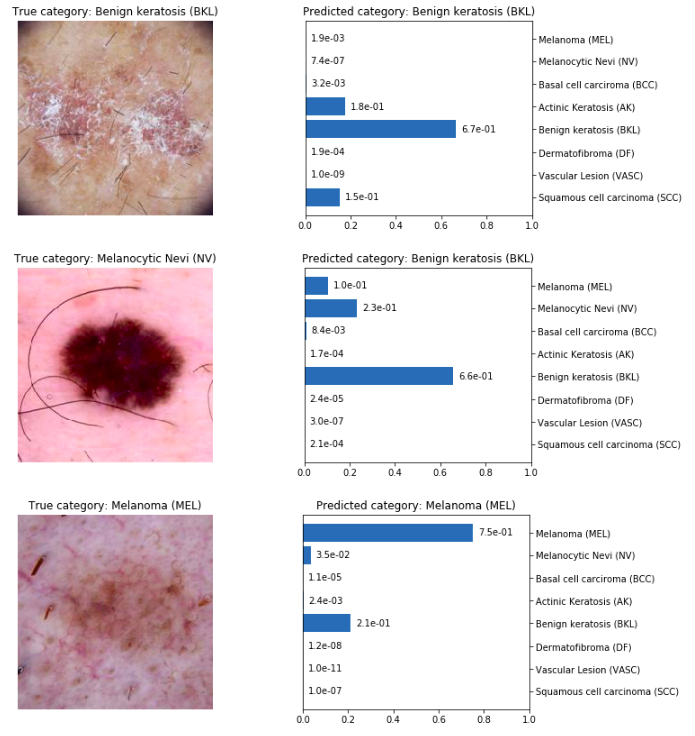
\includegraphics[width=\textwidth]{figs/Softmax_probs.png}
        \caption[Three samples of the test set along with their respective softmax probabilities.]{3 Samples of the test set along with their respective softmax probabilities. Results were inferred using the fine-tuned DenseNet201 model.}
        \label{fig:softmax_examples}
    \end{figure}
    
    \subsection{Freeze the Convolutional Layers}
    One way of re-purposing a pre-trained model is by simply replacing its classifier. For this procedure, the top layers of the pre-trained model must be removed, which are the layers that are not convolutional or pooling layers at the end of the pre-trained model's architecture (also called the convolutional base). Additionally, the weights from the layers of the convolutional base must be extracted and frozen, which means that they will be transferred directly from their original model and remain unchanged for the duration of the training process. Figure \ref{fig:pre_trained_models_classifier_comp} compares the accuracy and \ac{BMA} of applying this approach to several pre-trained models over the test set. One can observe that the overall performance is not optimal for any of the models, with the best performing architectures being VGG and EfficientNet. These results are to be expected because the weights of the layers in the convolutional base of these models were all trained in a very different dataset (ImageNet), from the \ac{ISIC} 2019 challenge dataset. \par
    \begin{figure}[ht]
        \centering
        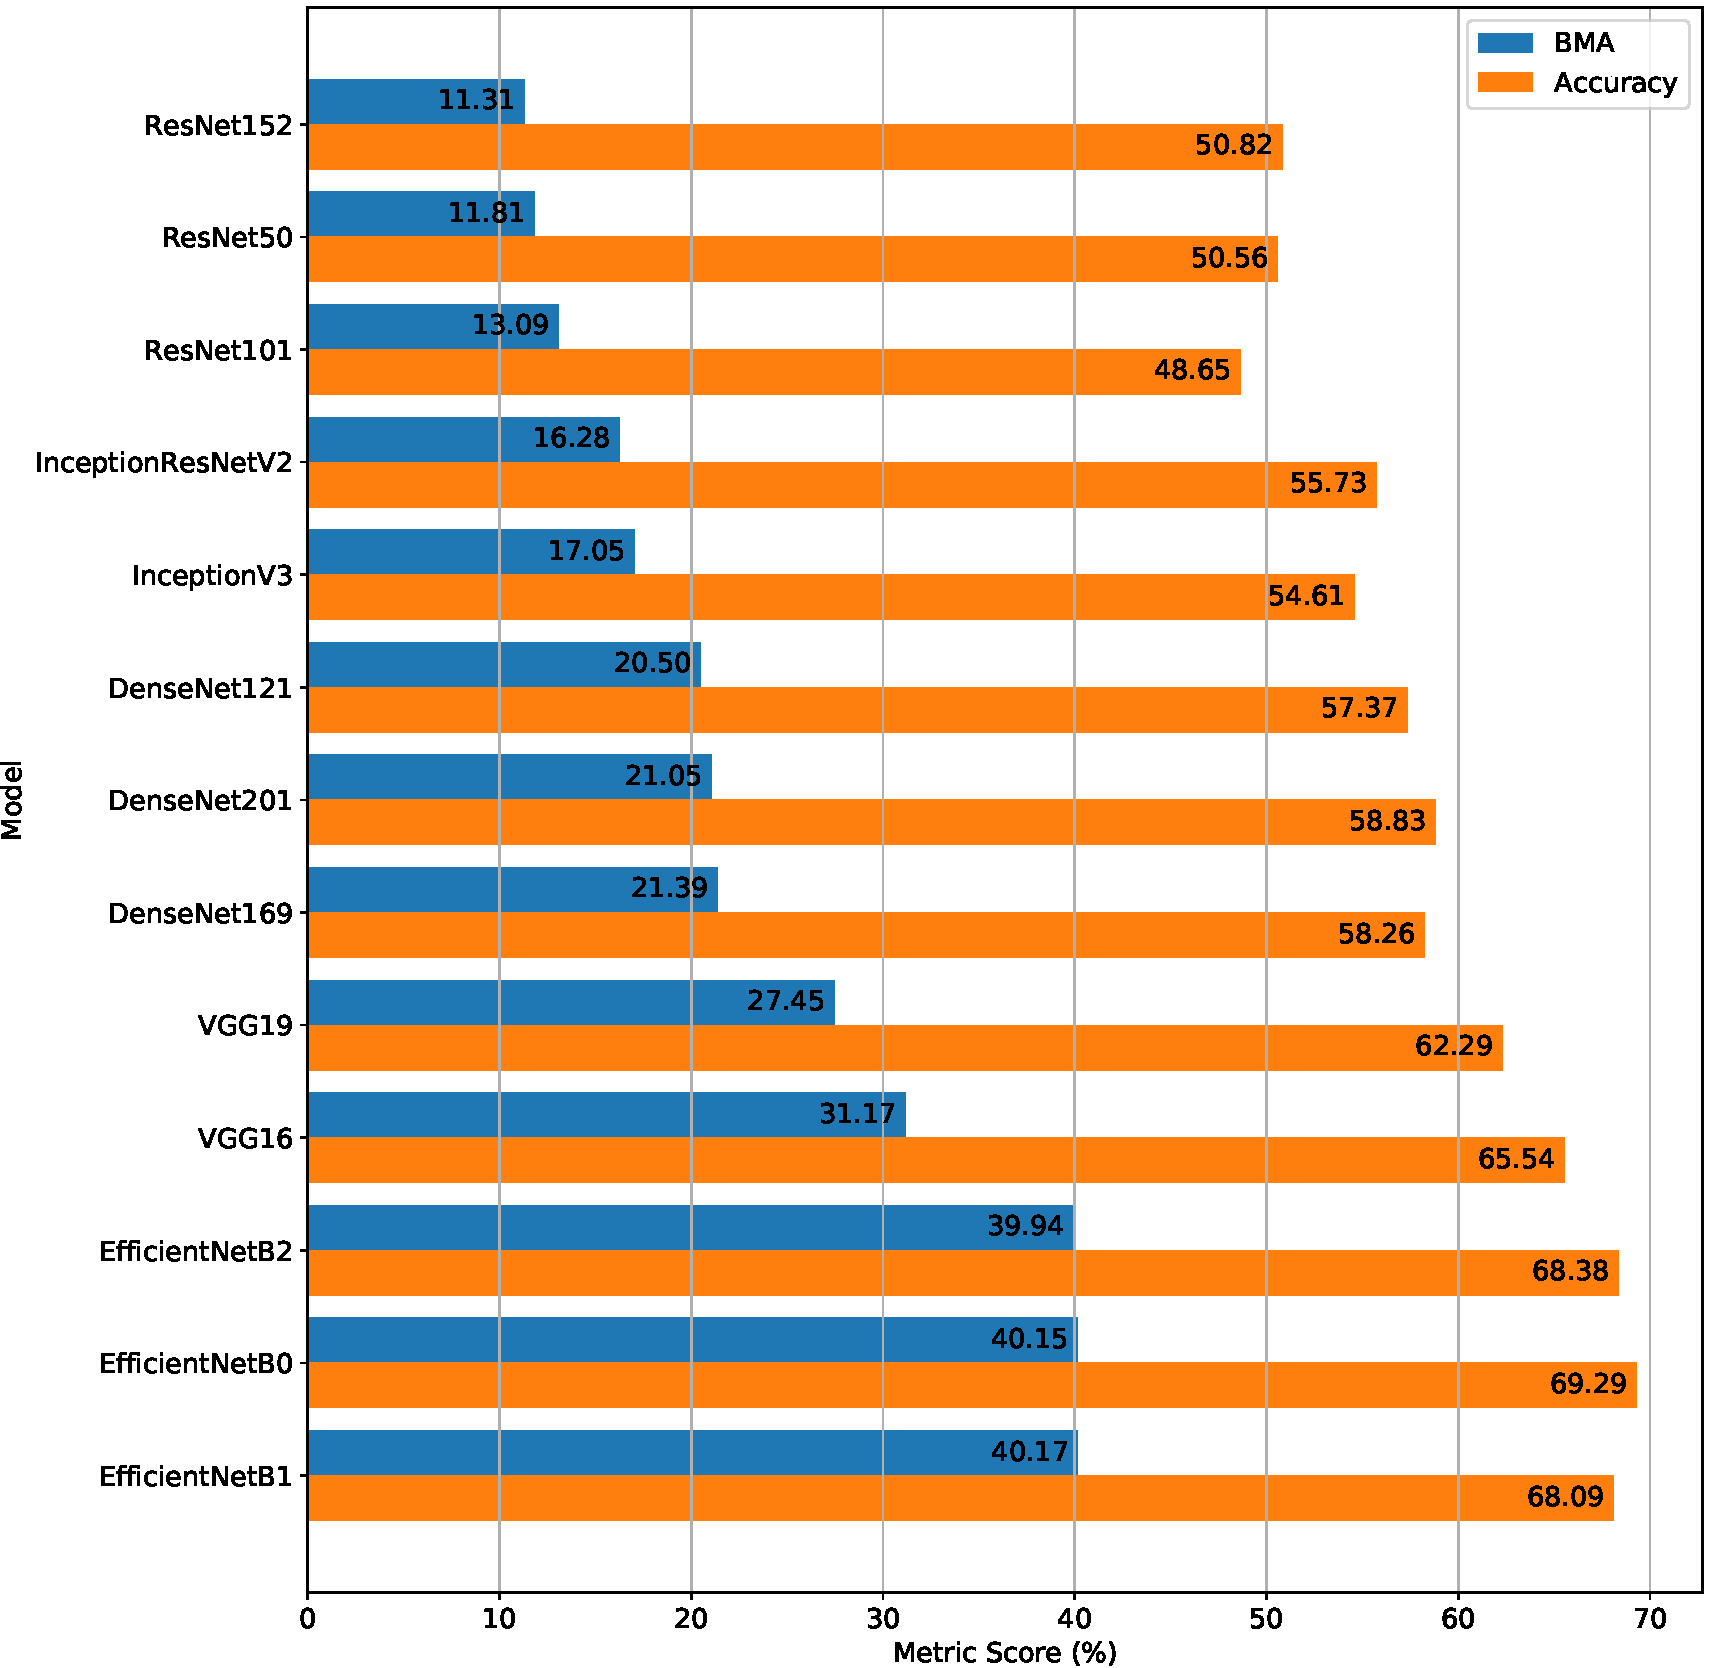
\includegraphics[width=0.9\textwidth]{figs/pre_trained_models_classifier_comp_horizontal.pdf}
        \caption[Comparison of pre-trained models with frozen convolutional base]{\ac{BMA} and Accuracy on the test set of multiple models pre-trained on ImageNet using transfer learning. Weights from convolutional layers are extracted from their initial model and frozen for the entirety of the training process. Classifier's layers are trained from scratch.}
        \label{fig:pre_trained_models_classifier_comp}
    \end{figure}
    
    Moreover, it seems like some model architectures are more capable of learning skin lesion related knowledge from only training the classifier. Namely, the EfficientNet family of models attains much better \ac{BMA} and accuracy scores in comparison with architectures like the ResNet or DenseNet. Presumably, the convolutional base of EfficientNets learns more generalizable knowledge in comparison with other architectures, which makes them more capable of achieving better performance using this transfer learning approach.  \par
    
    \subsection{Extraction and Fine-tuning of Convolutional Layers}
    Another approach is to adapt the whole set of parameters to this new dataset while also taking advantage of the already existing weights trained on ImageNet. This approach is based on the fine-tuning concept, meaning that all the weights from the pre-trained model are transferred to the new model (weight extraction), but are also updated along with the classifier on each epoch (unfrozen). Presumably, by taking this approach, the knowledge obtained from the existing weights will be adapted to a new problem and increase performance results on the test set. Figure \ref{fig:pre_trained_model_val_comp} shows that this assumption is true, as all pre-trained model achieve a significant increase in both accuracy and \ac{BMA} when compared with \autoref{fig:pre_trained_models_classifier_comp}. \par
    \begin{figure}[ht]
        \centering
        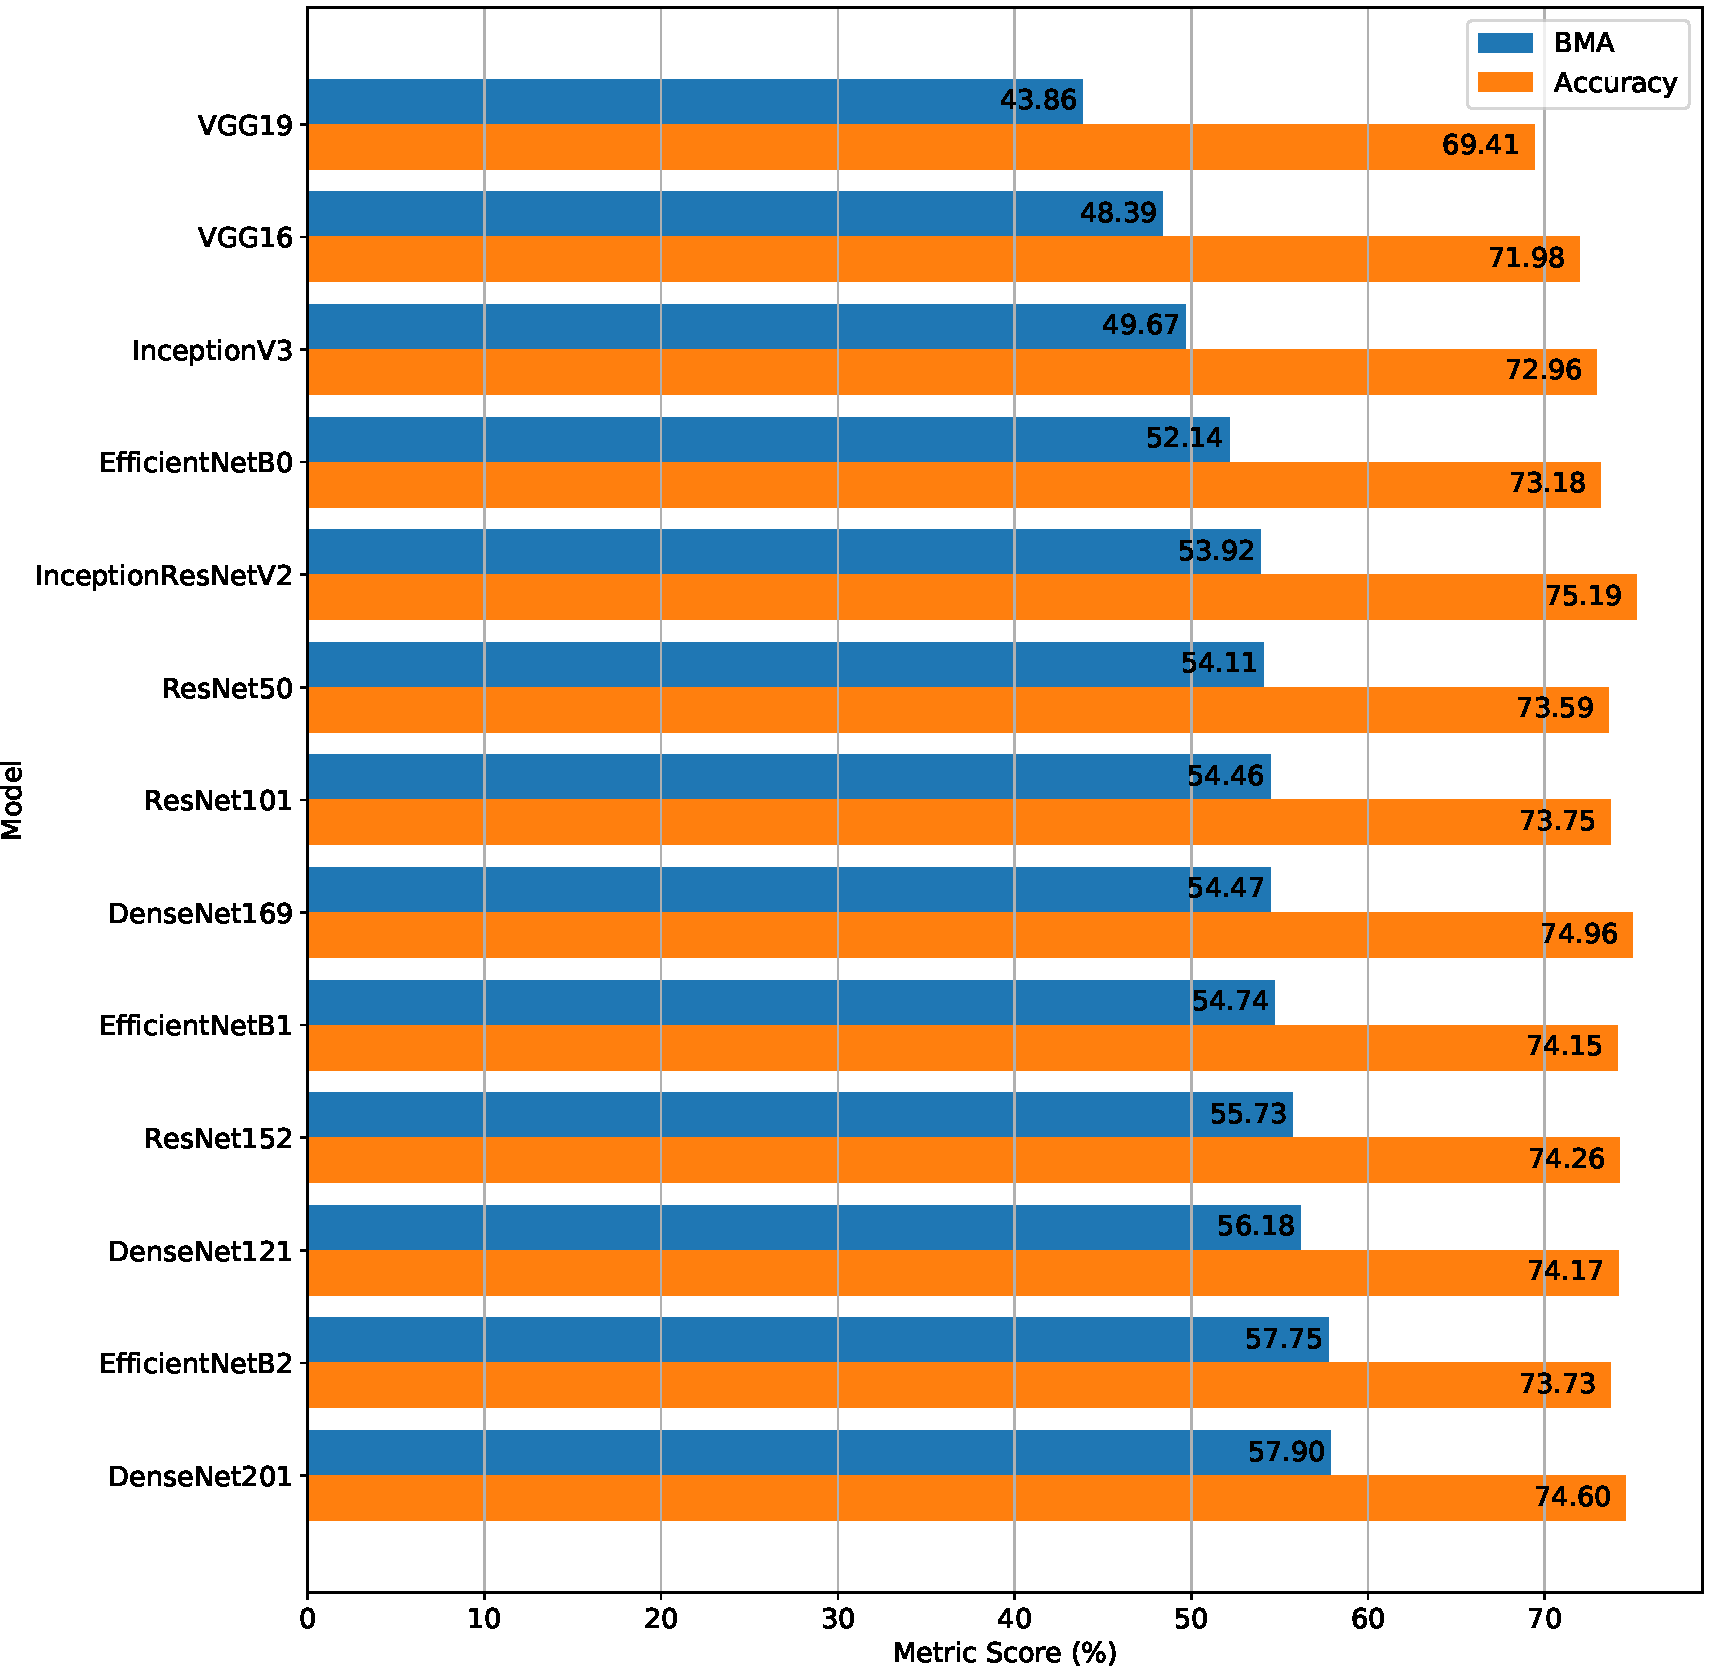
\includegraphics[width=0.9\textwidth]{figs/pre_trained_models_ft_comp_horizontal.pdf}
        \caption[Comparison of pre-trained models with fine-tuned convolutional base]{\ac{BMA} and Accuracy on the test set of multiple models pre-trained on ImageNet using transfer learning. Weights from convolutional layers are extracted from their initial model and fine-tuned for the entirety of the training process. Classifier's layers are trained from scratch.}
        \label{fig:pre_trained_model_val_comp}
    \end{figure}
    
    Generally by looking into \autoref{fig:pre_trained_model_val_comp}, one can observe that more recent architectures such as DenseNet or EfficientNet outperform older architectures such as VGG (see \autoref{tables:pretrainedmodels}). This can be attributed to the fact that the VGG16 and the VGG19 are shallower models compared to the others. It is to be expected that deeper models have a positive impact on model accuracy because more layers can create more levels of abstraction. The one exception to the depth rule is presented by the VGG family of models, which does not improve performance with depth increase (\textit{i.e.}, VGG16 and VGG19), presumably, related to the vanishing gradients problem. This is an issue that happens during the backpropagation of gradients while training, in which the gradient decreases exponentially as it gets propagated down to the initial layers \cite{Nielsen2017a}. When undealt, this issue becomes a larger concern for deeper networks like the VGG19. \par 
    
    This problem was later addressed by architectures such as ResNet with the introduction of the skip connection (see \Cref{section:cnn_archs}), which would allow it to create deeper models. Indeed, by looking at \autoref{fig:pre_trained_model_val_comp}, ResNet pre-trained models outperform older and shallower pre-trained models such as the VGG16 and VGG19. Even within the same architecture, ResNet takes advantage of the depth to further increase performance. DenseNet extended the skip connection concept which allowed it to build even deeper models such as the DenseNet201 with 201 layers. One can observe that the DenseNet pre-trained models outperform most of ResNet, VGG, and Inception pre-trained models, with the DenseNet201 being the best performing pre-trained model. \par
    
    From looking at \autoref{fig:pre_trained_model_val_comp}, EffcientNets scale exceptionally well with the amount of trainable parameters available. For example, EfficientNetB0, which is the model with less trainable parameters from all the tested models, has similar performance to the InceptionResNetV2 which has a much larger amount of trainable parameters (see \autoref{tables:pretrainedmodels}). In contrast, EfficienNetB2 has similar test set performance to the DenseNet201, while having a considerably lower amount of trainable parameters. One can hypothesize that the scalability of this family of models concerning the number of trainable parameters is related to the compound scaling method presented by Tan \textit{et al.} \cite{efficientnet} (see \Cref{section:cnn_archs}). Moreover, one can assume that bigger models such as the EfficientNetB3 or even the EfficientNetB7 could outperform DenseNet201. However, it has been decided not to train and test such models, because of the limited compute capability of Deeplar (see \Cref{section:hardware}). \par 
    
    Furthermore, one can observe that for all the pre-trained models, the \ac{BMA} is much lower than the accuracy. This is a consequence of the train and test sets being imbalanced, which makes the model correctly classify more samples towards classes with more data (illustrated in \autoref{fig:densenet201_pred_dist}). The accuracy metric is very sensitive to this type of imbalance, as it does not give the same weight to each class's performance. For the accuracy metric, the weight of each class is proportional to the number of samples of that class on the test set, which makes it very prone to increase or decrease according to the performance of overrepresented classes. In contrast, for the \ac{BMA} score, the performance of the model in each class is weighted the same (see \cref{section:metrics}), which substantially lowers the score because underrepresented classes have significantly worse performance than overrepresented classes. \par
    \begin{figure}[ht]
        \centering
        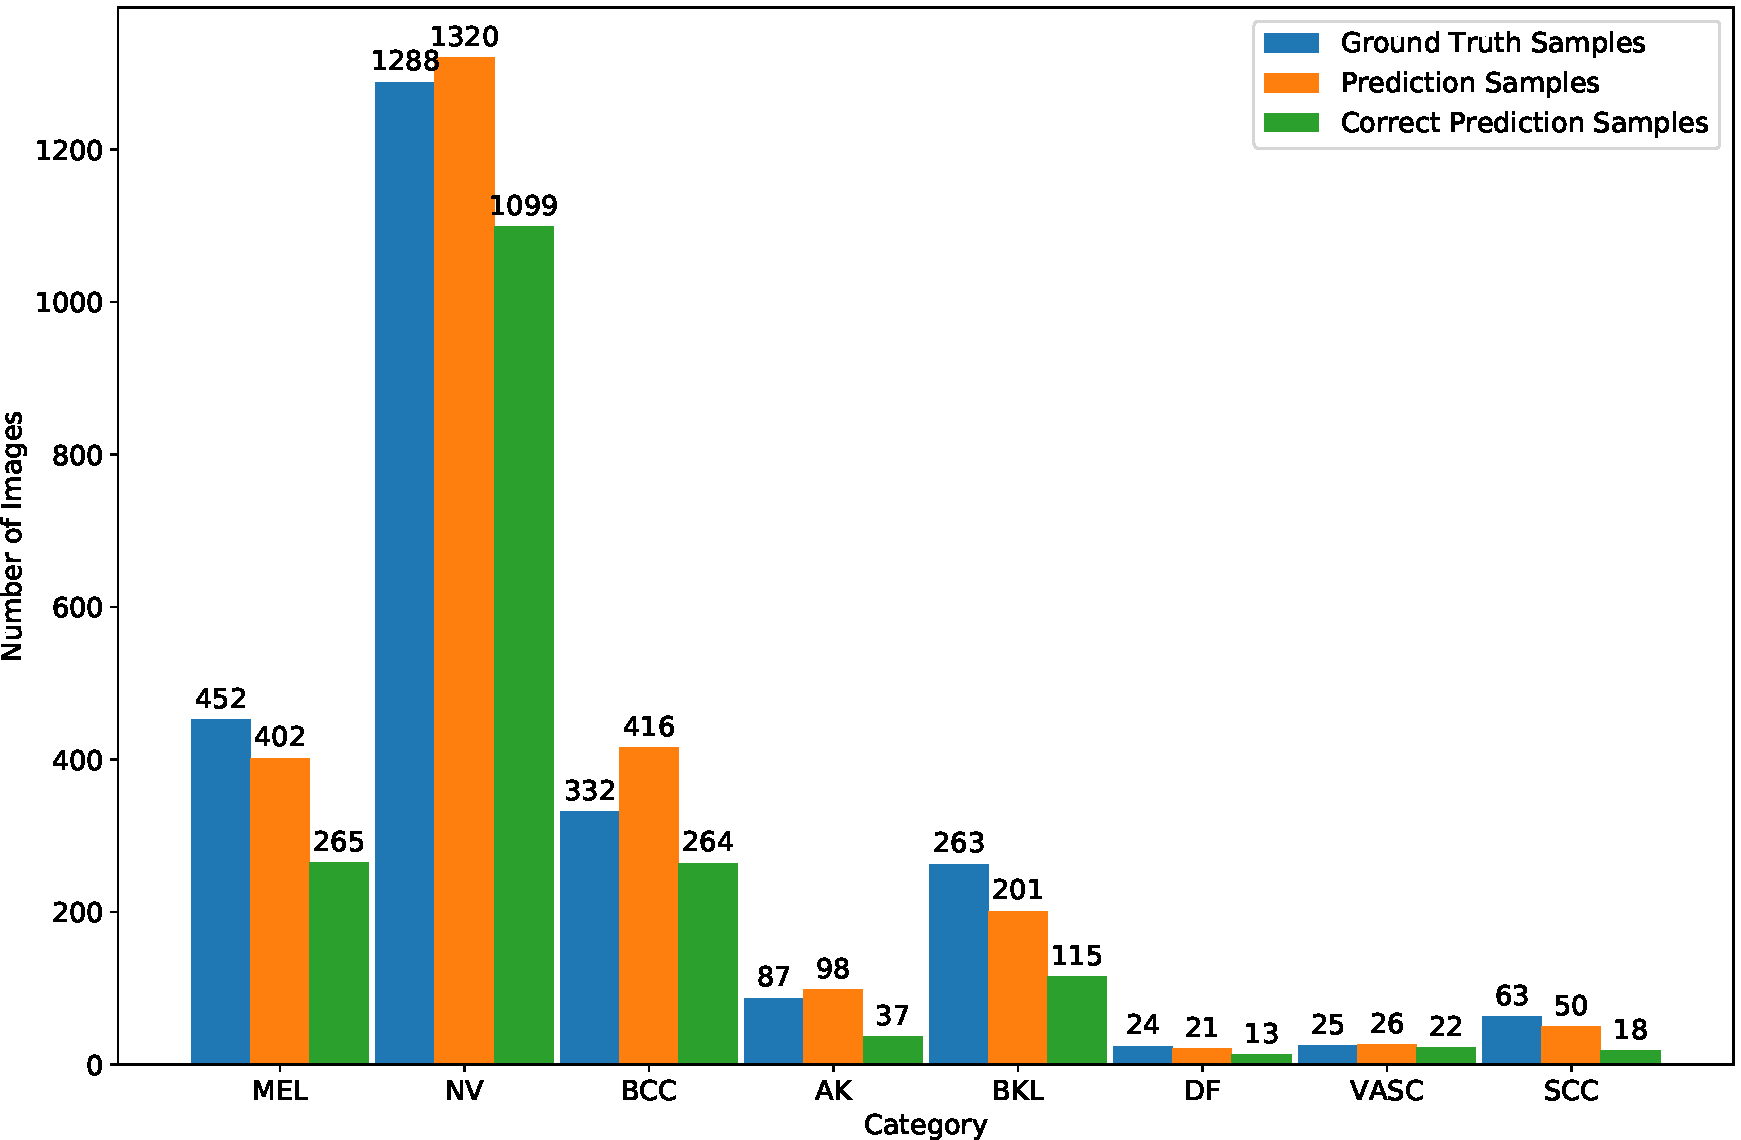
\includegraphics[width=\textwidth]{figs/densenet201_pred_dist.pdf}
        \caption{Ground truth samples, prediction samples, and correct prediction samples across different classes in the test-set using the fine-tuned DenseNet201 model.}
        \label{fig:densenet201_pred_dist}
    \end{figure}

\section{Hyperparameter Optimization} \label{section:hyperparameters}
    So far, models were trained with commonly used hyperparameters from the approaches for the \ac{ISIC} 2019 presented in \Cref{chapter:sota}. However, as a means to optimize these values, one should carefully analyze and test different hyperparameters values, to hopefully improve the test set performance. Therefore, in this section, results from a multitude of experiments with different hyperparameters will be presented. \par
    
    In order to systematically optimize each hyperparameter without leading to a combinatorial explosion, the following strategy is employed:
    \begin{itemize}
        \item For each hyperparameter, a range of common values from the literature are tested and compared with one another using train and validation \ac{BMA};
        \item The choice of the hyperparameter is made according to an analysis of the results, and all subsequent experiments with other hyperparameters will use that choice;
        \item This process will be repeated until all hyperparameters are chosen. 
    \end{itemize}
    
    Taking this into consideration, a benchmark for each experiment will be set to fairly compare different hyperparameters and to take advantage of the already acquired knowledge from \Cref{section:models}. More specifically:
    \begin{itemize}
        \item Each model is trained on an undersampled version of the \ac{ISIC} 2019 dataset with 5000 training samples, that maintains the original class distribution. The undersampling process is done by randomly selecting samples from the original dataset in a stratified manner. This smaller dataset will substantially decrease each model train time, which will allow us to experiment with more hyperparameters in an agile way. An undersampled version of the original dataset will likely yield similar conclusions as if the whole dataset was being used;
        \item Online data augmentation is performed with crops, flips, and rotations to reduce overfitting while training;
        \item For the transfer learning approach, all the layer's parameters from the convolutional base of the pre-trained model are extracted and fine-tuned, which yields the best performance for this specific dataset (see the results presented in \Cref{section:models});
        \item An global average pooling layer is introduced at the end of the convolutional base in order to reduce the number of parameters for the classifier;
        \item The original pre-trained model's classifier is replaced by a new classifier composed of one fully-connected layer with 512 neurons which use the ReLU activation function, and one softmax layer with 8 neurons to translate each of the class's probabilities;
        \item The classifier weights are initialized using Glorot's initialization \cite{Glorot2010};
        \item Following the work done by Gessert \textit{et al.} \cite{gessert2018} the Adam optimizer \cite{adam} is used, with $\rho_{1} = 0.9$ and $\rho_{2}=0.999$;
        \item Each model trains for a maximum of 100 epochs but early stopping is performed whenever validation loss stops improving for 16 epochs, as a measure to reduce overfitting;
        \item For each epoch, all the samples are shuffled before being feed into the network;
        \item For each training process, 3 models are saved: The model that obtained the highest \ac{BMA} on the validation set, the model with the lowest loss on the validation set, and finally the resulting model from the last epoch. However, performance is always evaluated according to the model which attained the highest \ac{BMA} on the validation set. 
    \end{itemize}
    
    \subsection{Varying the Batch Size}
    The batch size defines the number of training samples passed through the network in one forward and backward pass. The batch size is directly correlated to the number of iterations per epoch using the \autoref{eq:iter_epoch}.
        \begin{equation}
        \mbox{iterations per epoch}=\frac{\mbox{number of samples}}{\mbox{batch size}}
        \label{eq:iter_epoch}
        \end{equation}
    where one iteration is one backward and forward pass. This means that larger batch sizes will have less iterations per epoch, which generally makes them faster to train. However, larger batch sizes also increase the \ac{GPU}'s memory requirements. \par
    
    Tests have been made for 4 different batch sizes, more specifically, 4, 8, 16, and 32. Larger batches than 32 are impractical for this experimental setup because Deeplar at \ac{LAR} (see \Cref{section:hardware}), runs out of memory on some pre-trained models with large batch sizes(\textit{e.g.}, InceptionResNetV2, DenseNet201). \par

    From the results in \autoref{fig:batch_comp}, one can observe that smaller batch sizes improve the \ac{BMA} scores on the validation set while also having a regularization effect, because train and validation \ac{BMA} scores are much closer together for smaller batch sizes (\textit{e.g} 4) in comparison with larger ones (\textit{e.g.}, 32). However, one should also consider the disadvantages of using such small batch sizes, namely, longer times to train the models, which can become troublesome with larger datasets such as the ones used further in \Cref{section:balance}. Therefore, as a compromise between agility and performance, a batch size of 8 was chosen for future experiments. \par
    
    \begin{figure}[ht]
        \centering
        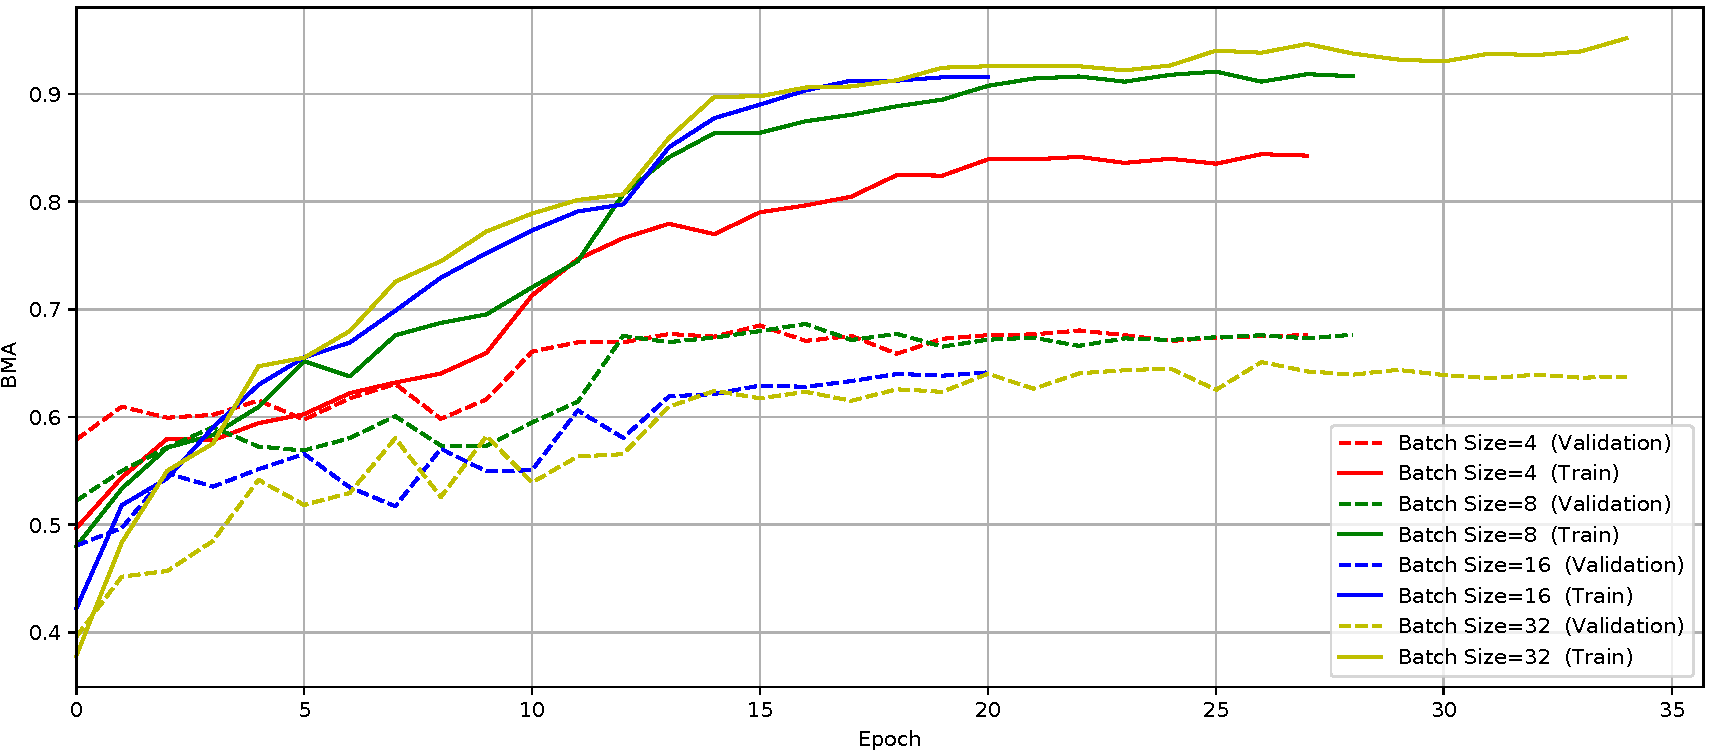
\includegraphics[width=\textwidth]{figs/densenet201_batch_over_epochs.pdf}
        \caption{Batch size vs train and validation \ac{BMA} over epochs for the fine-tuned DenseNet201 trained with 5000 samples.}
        \label{fig:batch_comp}
    \end{figure}  
    
    \subsection{Varying the Number of Epochs Before Fine-Tuning}
    One important aspect of training deep neural networks is the number of epochs that it will run on. One epoch is when all training examples have been forward and backward passed through the network. More specifically, in one epoch all image samples are fed to the network in several iterations given by \autoref{eq:iter_epoch}. Therefore, the number of epochs defines how many times each image is seen by the network. The maximum number of epochs has been fixed to 100, but most of the tested models never reach that point because of early stopping. \par
    
    In this approach to transfer learning, the pre-trained model's classifier is replaced by an untrained one, which means that the classifier's weights are initially defined by the Glorot's initialization method \cite{Glorot2010}. Knowing that the initial weights of the classifier are determinant for the overall model performance, one can hypothesize that by freezing the convolutional base for an initial number of epochs and only train the classifier weights for that amount of time, will lead to better converge point during the training process. Therefore, in this process, the classifier's weights are being adapted to the new dataset, before the actual fine-tuning process starts. \par
    
     \par
    \begin{figure}[ht]
        \centering
        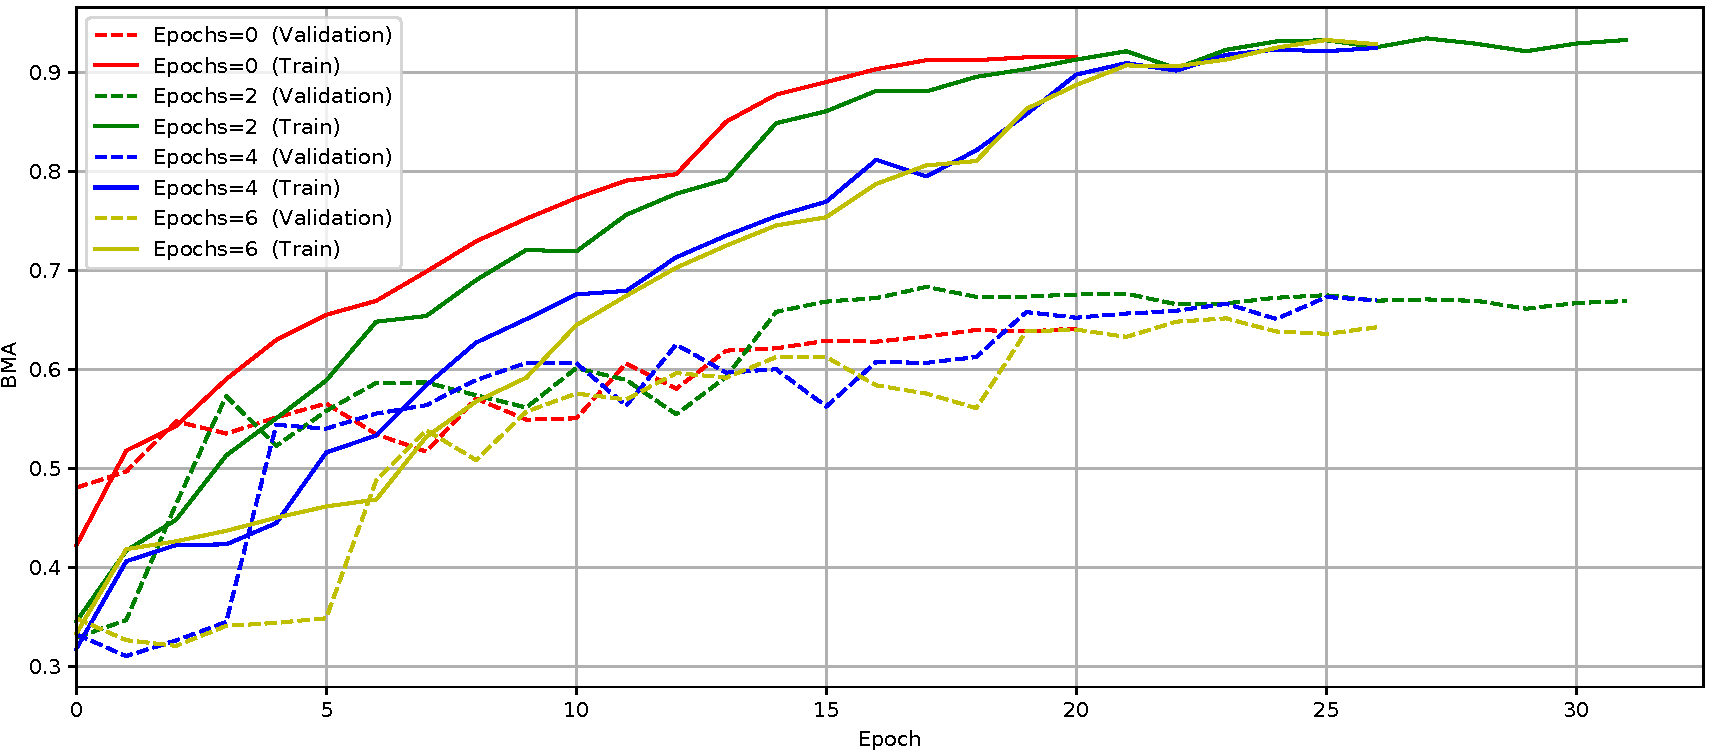
\includegraphics[width=\textwidth]{figs/densenet201_wiepochs_over_epochs.pdf}
        \caption{Number of epochs before the fine-tuning process vs train and validation \ac{BMA} over epochs for the fine-tuned DenseNet201 trained with 5000 samples.}
        \label{fig:wiepochs_comp}
    \end{figure}
    
    Figure \ref{fig:wiepochs_comp} illustrates the impact of different numbers of epochs used to train the classifier before the fine-tuning process starts, on the overall performance. Results show that by using this method, models start to significantly improve \ac{BMA} later, but generally train for more epochs and reach better converge points. For example, if one uses 0 epochs during this phase (immediately start the fine-tuning process), the model stops on epoch 20 in a rather worse convergence stop in comparison with using 2, 4 or even 6 epochs, which end the training process at the 31th, 26th and 26th epoch, respectively. \par
    
    However, there are no significant improvements to be shown by using 4 or 6 epochs before the fine-tuning process starts in comparison with 2, as all of them end up with similar, if not worse, \ac{BMA} scores. Therefore, the remaining experiments will use 2 epochs to train the classifier before the fine-tuning process of the convolutional base. \par
    
    \subsection{Varying the Learning Rate}
    \label{section:lr_tune}
    Presumably, the most important hyperparameter to optimize is the learning rate. It controls the step size for model weight updates concerning the loss function. Lower values mean slower travel along the downward slope but consequently take more epochs to converge into a local minimum. In this approach, two learning rates are considered, namely, the learning rate used before the fine-tuning process starts and the initial fine-tuning learning rate. \par 
    
    Some experiments have been done to define which learning rate to use during the phase in which only the classifier is trained, more precisely, before the fine-tuning of the convolutional base process starts. Results in \autoref{fig:wilr_comp} show that the model benefits from having larger learning rates during this phase, which presumably stems from the fact that the classifier's weights are not adapted to the \ac{ISIC} 2019 dataset. Therefore, one can assume that using larger learning rates to adapt the classifier to the new dataset will ultimately lead to a better converge point by the end of the training process. As such, the learning rate used to only train the classifier before the fine-tuning process starts will be $10^{-3}$ for the remaining experiments. \par
    \begin{figure}[ht]
        \centering
        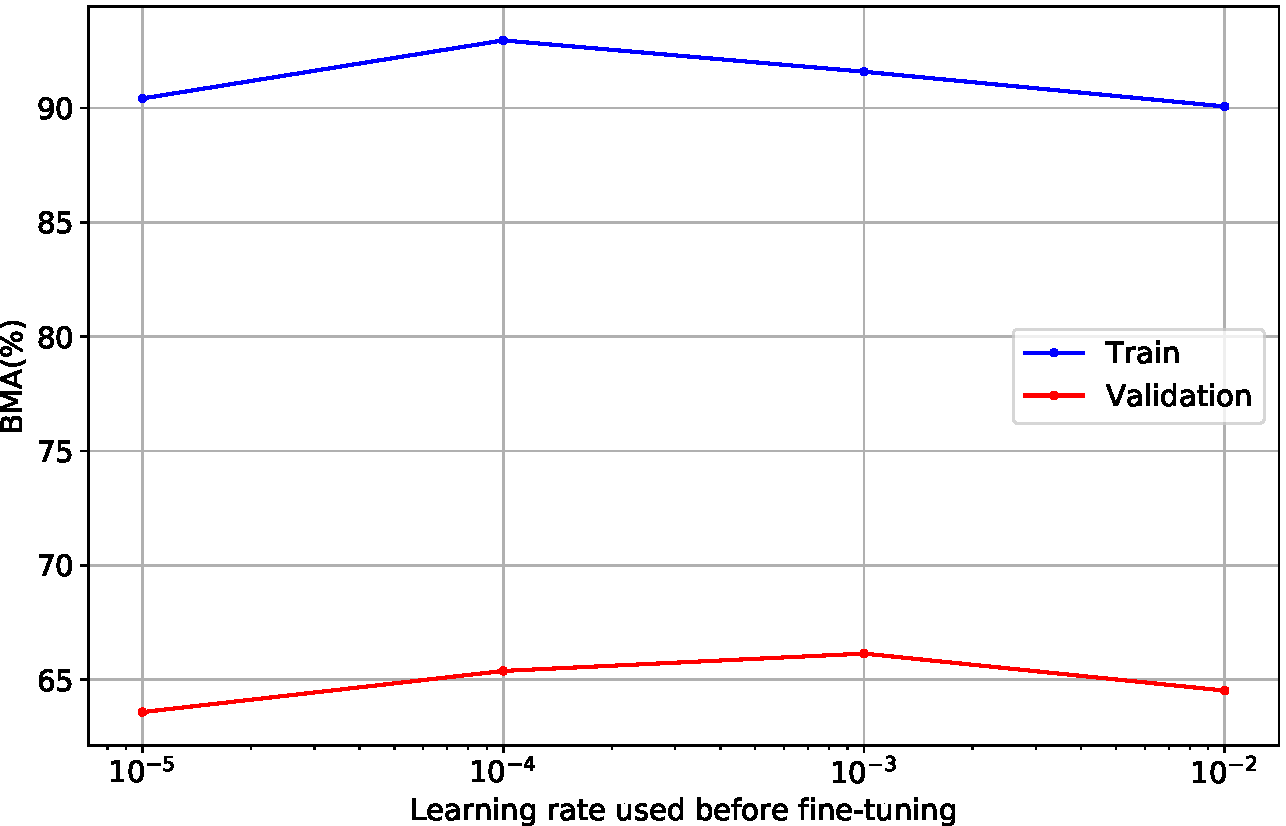
\includegraphics[width=0.7\textwidth]{figs/densenet201_wilr_comp.pdf}
        \caption{Learning rate used to train the classifier before the fine-tuning process vs \ac{BMA} for the fine-tuned DenseNet201 trained with 5000 samples.}
        \label{fig:wilr_comp}
    \end{figure}
    
    Furthermore, there is a far more important learning rate which one can call the initial fine-tuning learning rate and it is used to fine-tune the whole model after the weights of the classifier had been initialized. Hypothetically, choosing too small learning rate values will result in a long training process that could get stuck in a local minimum, whereas a value too large may result in learning a sub-optimal set of weights too fast or an unstable training process. One can verify this hypothesis by comparing various fine-tuning learning rates in \autoref{fig:ftlr_comp}. \par
    \begin{figure}[ht]
        \centering
        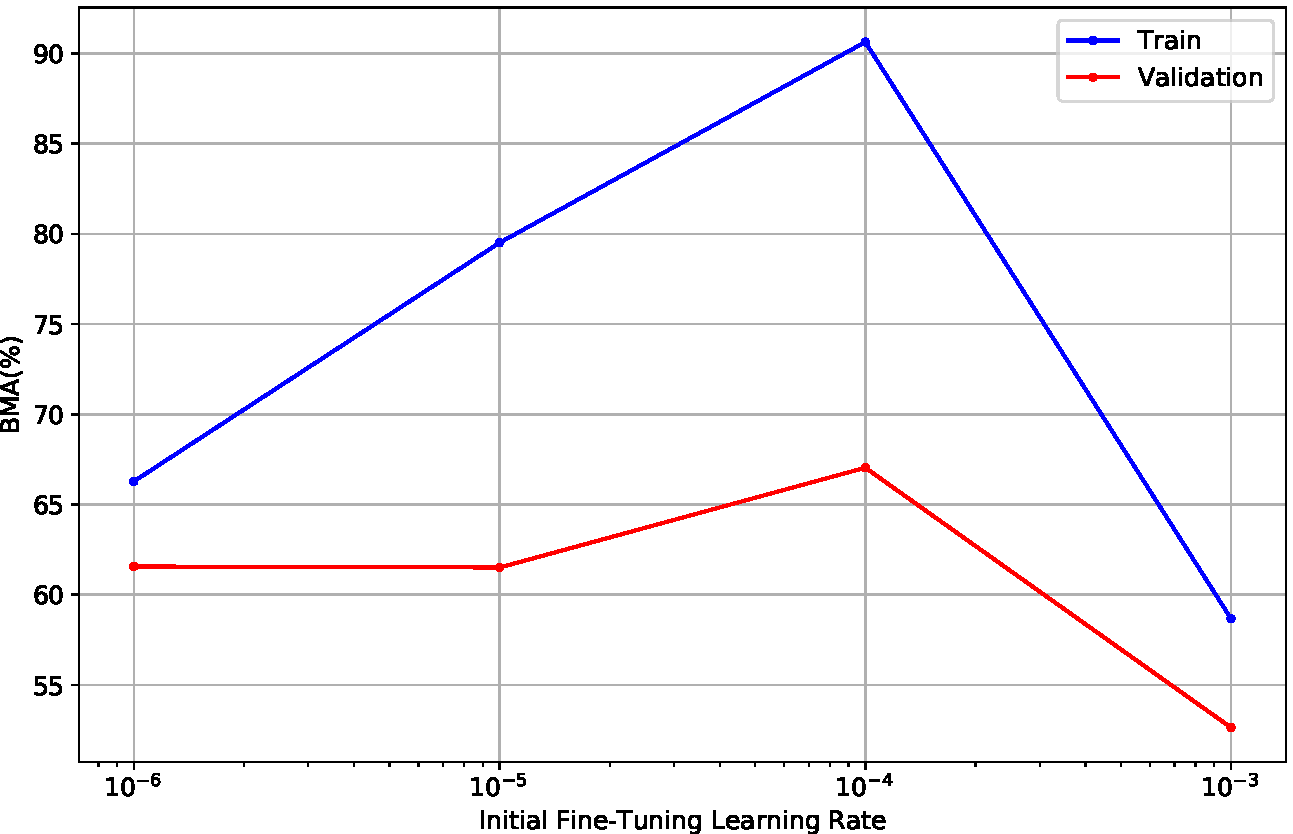
\includegraphics[width=0.7\textwidth]{figs/densenet201_ftlr_comp.pdf}
        \caption{Fine-tuning learning rate vs train and validation \ac{BMA} for the fine-tuned DenseNet201 trained with 5000 samples.}
        \label{fig:ftlr_comp}
    \end{figure}
    
    Figure \ref{fig:ftlr_bma_over_epochs} shows that a low learning rate like $10^{-6}$ makes the improvements linear, while higher learning rates like $10^{-4}$ tend to show a more exponential curve because they will decay the loss faster. However, when the learning rates are too big they can get stuck at worse values of loss which is the case of $10^{-3}$. This is because there is too much "energy" in the optimization and the parameters are bouncing around chaotically, unable to settle in a good spot in the optimization landscape. \par
    
    The learning rate of $10^{-4}$ seems to be the optimal choice because it allows the model to have a higher chance of finding a better region of search space in the initial epochs, which consequently influences the rest of the training process. After all, the rest of the epochs will be spent on minimizing the loss within that specific region, which is finding the local minimum. In contrast, learning rates like $10^{-5}$ and $10^{-6}$ have a lower chance of finding a good local minimum at the beginning of the training process, and therefore take more epochs to converge. Higher learning rates like $10^{-3}$ are too big, which leads to the network never finding a good region of search space at the beginning of the training process, and ultimately jumping between convergence stops. \par
    
    \begin{figure}[ht]
        \centering
        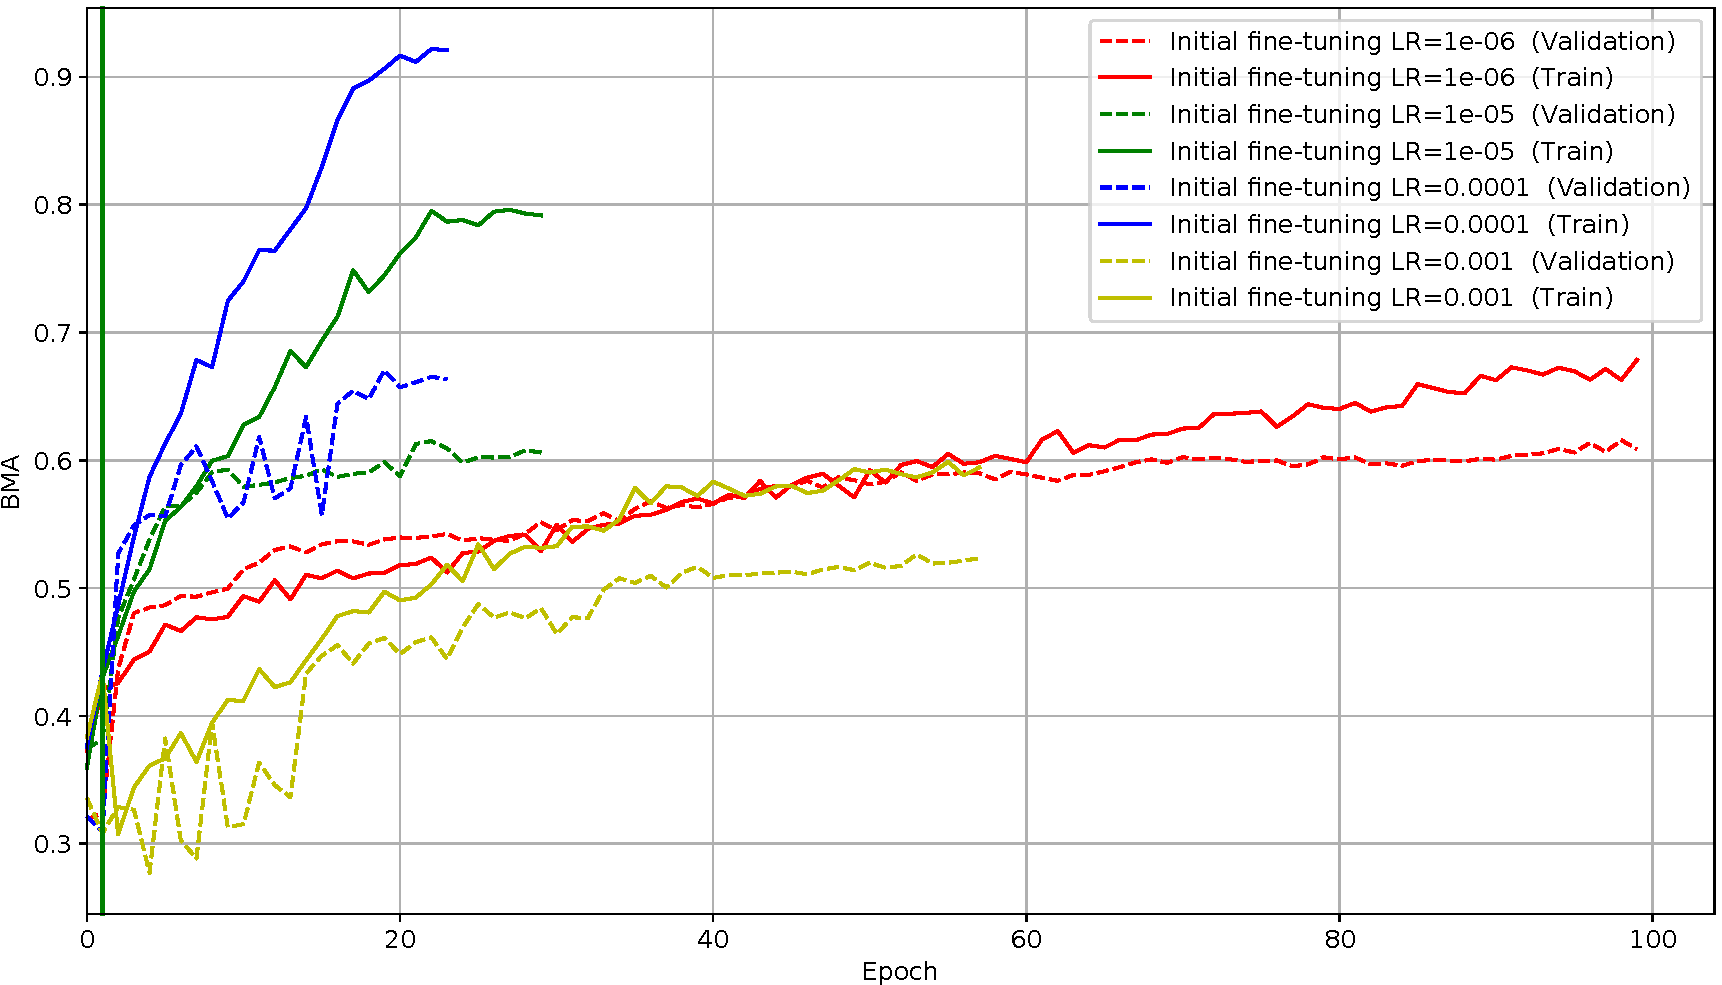
\includegraphics[width=\textwidth]{figs/densenet201_ftlr_bma_over_epochs.pdf}
        \caption{Influence of the fine-tuning learning rate on train and validation \ac{BMA} over epochs for the DenseNet201 trained with 5000 samples.}
        \label{fig:ftlr_bma_over_epochs}
    \end{figure}
    
    One can also observe the influence of the learning rate scheduler by looking at \autoref{fig:ftlr_lr_over_epochs}. A low learning rate like $10^{-6}$ is not affected by the learning rate scheduler as it keeps the same global learning rate across the whole training process. This happens because the validation loss keeps slowly decreasing (see \autoref{fig:ftlr_loss_over_epochs}) until it reaches the maximum number of epochs. In contrast, high initial fine-tuning learning rates like $10^{-3}$ have a step curve evolution of the learning rate coming down until it reaches a local minimum at $10^{-3}$. However, using such a learning rate will make the weight updates overshoot good convergence points as seen by the highs and lows of the validation loss curve. \par  
    
    \begin{figure}[ht]
        \centering
        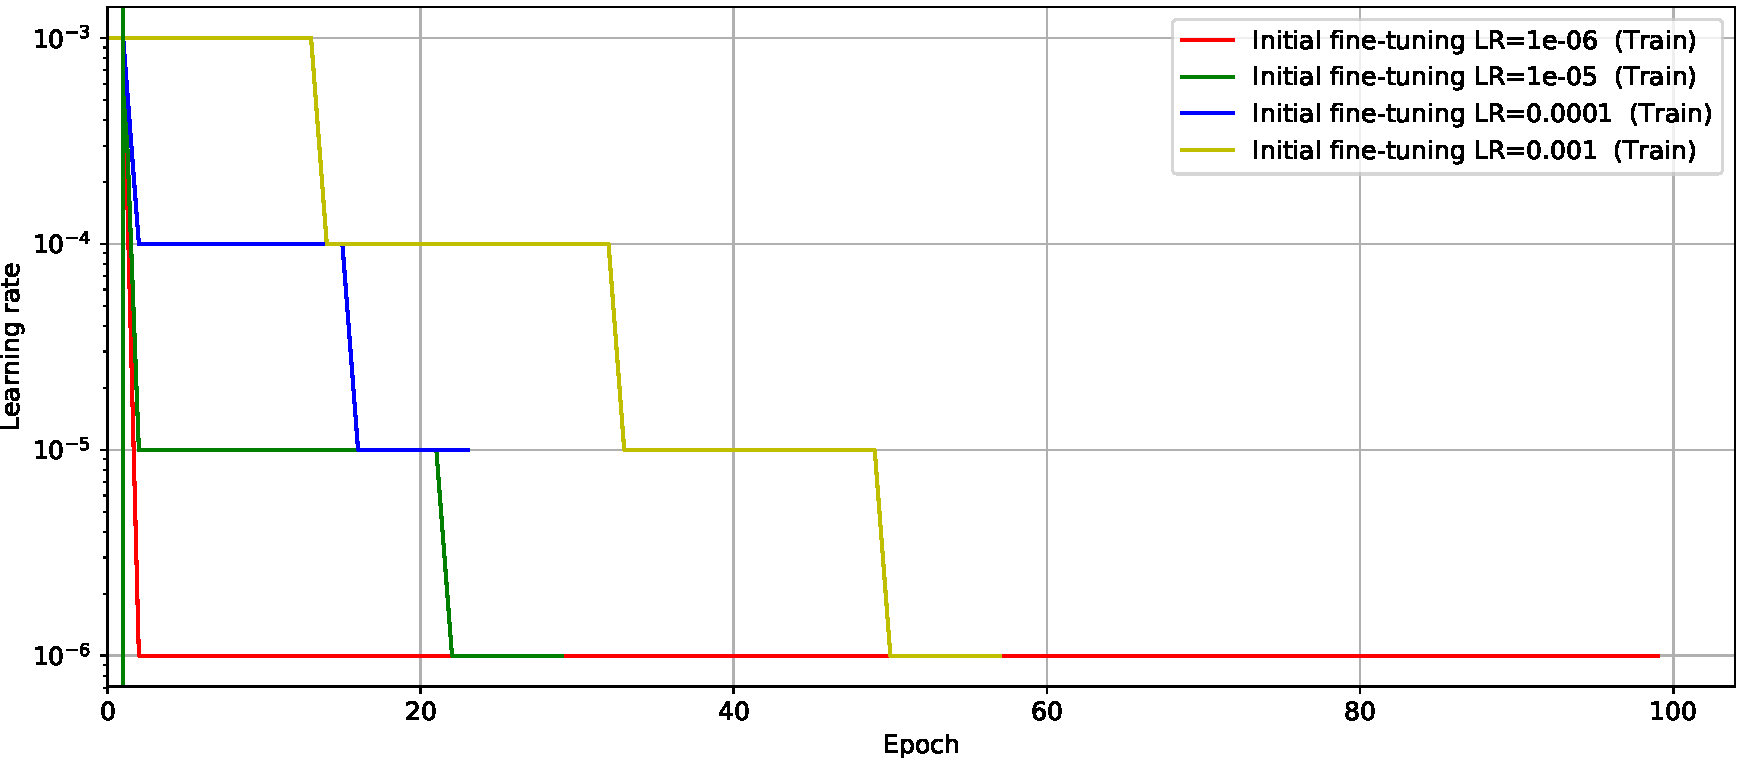
\includegraphics[width=\textwidth]{figs/densenet201_ftlr_lr_over_epochs.pdf}
        \caption{Initial fine-tuning learning rate vs the learning rate over epochs for the DenseNet201 trained with 5000 samples.}
        \label{fig:ftlr_lr_over_epochs}
    \end{figure}
    
    Moreover, even though the learning rate of $10^{-4}$ does not decrease in a step-like manner like $10^{-3}$ (see \autoref{fig:ftlr_lr_over_epochs}), it converges much more rapidly to a local loss minimum earlier during training as seen by the loss curve in \autoref{fig:ftlr_loss_over_epochs}. The initial fine-tuning learning rate of $10^{-5}$ can also be a good option as it converges quickly to a similar loss point. However, considering the results \autoref{fig:ftlr_comp}, it is clear that $10^{-4}$ is the better option, so it will be used for the remaining experiments. \par
    
    \begin{figure}[ht]
        \centering
        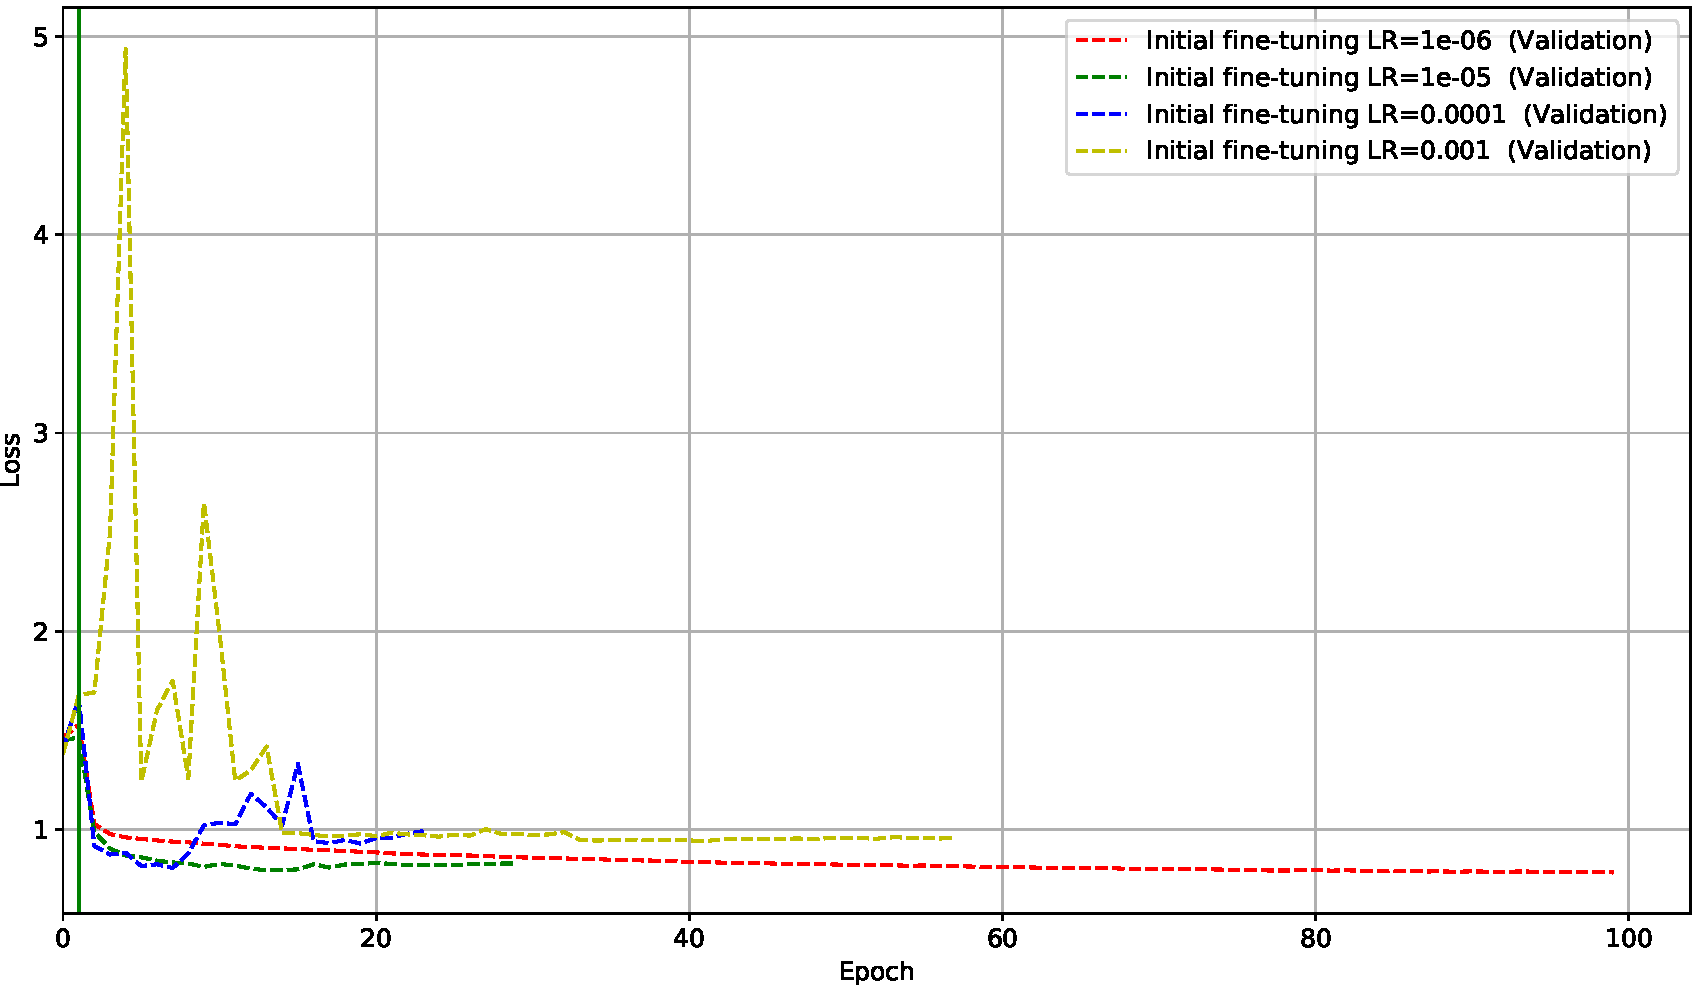
\includegraphics[width=\textwidth]{figs/densenet201_ftlr_val_loss_over_epochs.pdf}
        \caption{Initial fine-tuning learning rate vs validation loss over epochs for the DenseNet201 trained with 5000 samples.}
        \label{fig:ftlr_loss_over_epochs}
    \end{figure}
    
    
    \subsection{Varying the Learning Rate Scheduler's Patience}
    During the training of deep neural networks, it is useful to reduce the learning rate as the number of training epochs increases. The intuition behind this concept is that with high learning rates, the deep learning model will make larger parameter updates. This is helpful during the early epochs because the model is searching for a convergence spot within a large number of possible combinations of parameters. However, in the latter stages of training, the intention is to find the optimal spot within a narrower search area rather than search for other convergence spots. Therefore, the parameter search during the latter stages of the optimization process is supposed to have a much narrower search domain than in the earlier stages. \par
    
    The learning rate schedulers usually have a hyperparameter called patience, which dictates how many epochs the training process should wait after no improvements were made within a predefined metric value. In this approach that metric is the validation loss, meaning that if the model does not decrease the validation loss for several epochs (patience), then the learning rate is decreased by a factor of 10. However, there is no clear value for the patience one model should have for the learning rate scheduler. It is hypothesized that high patiences will lead to chaotic improvements throughout the training process, but low patiences will eventually lead to premature early stopping. \par
    
    \begin{figure}[ht]
        \centering
        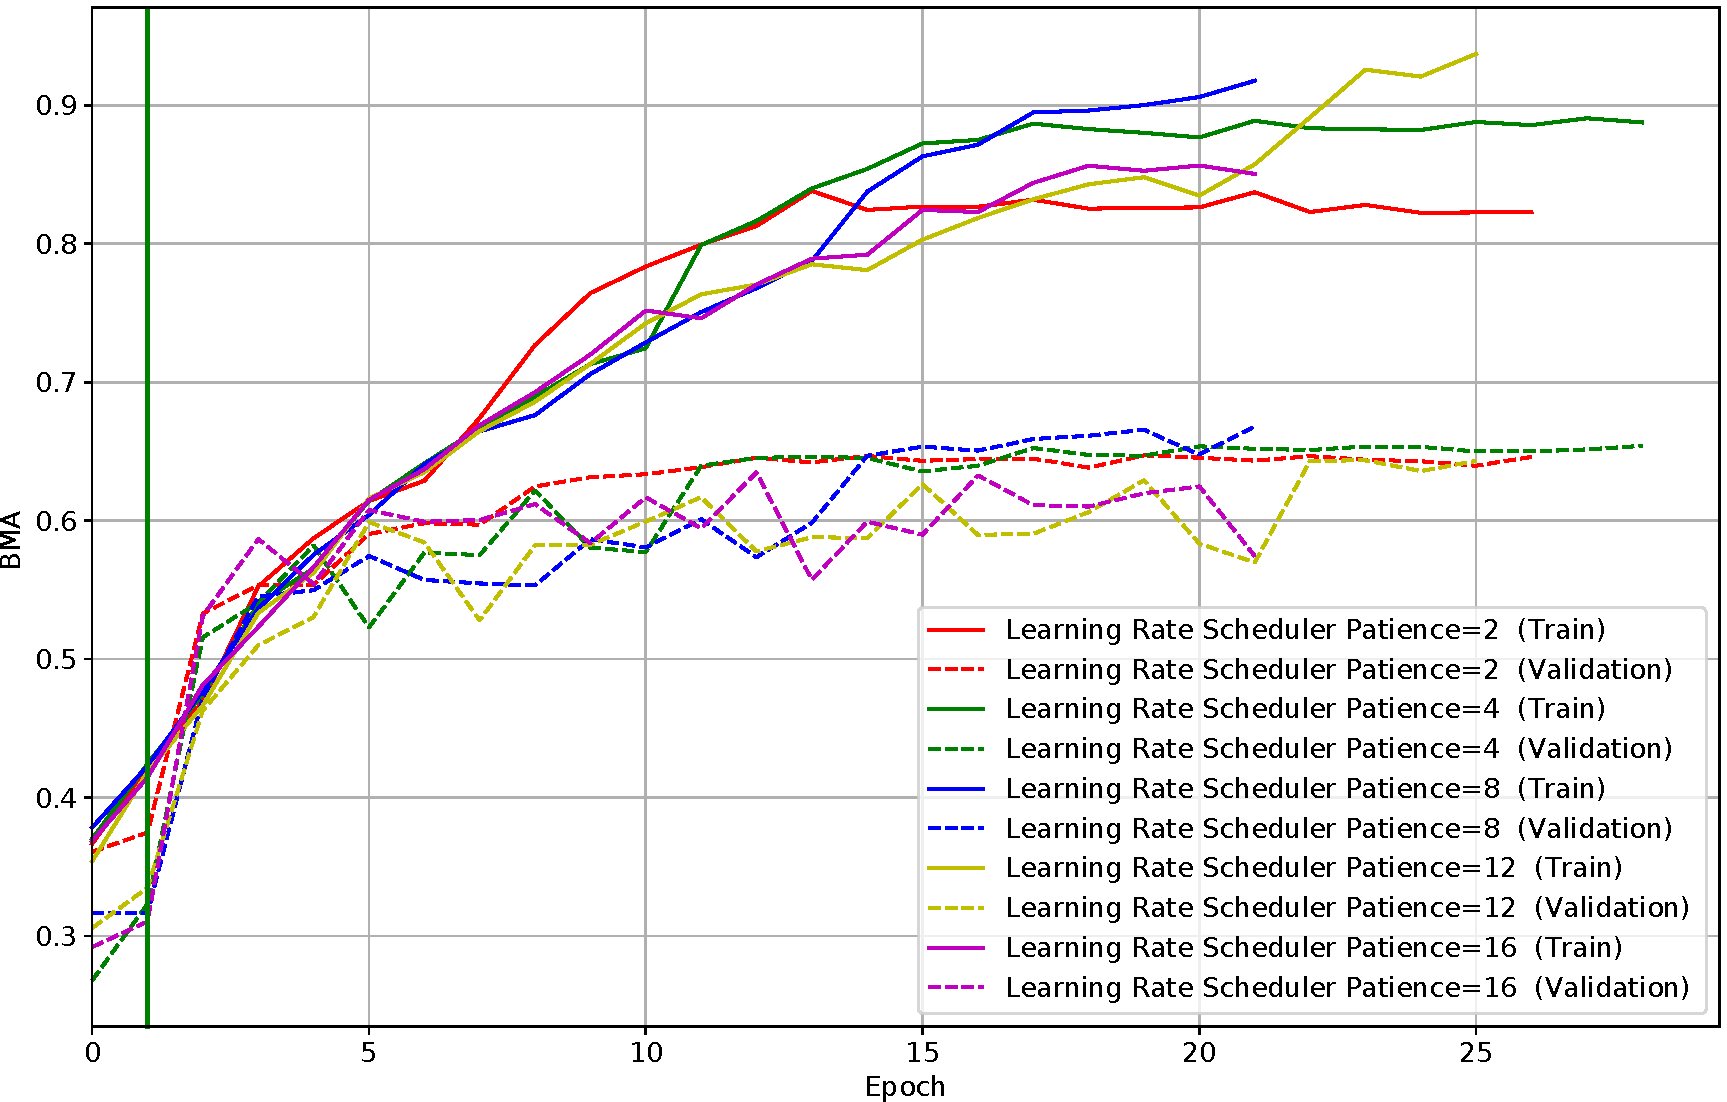
\includegraphics[width=\textwidth]{figs/densenet201_patience_over_epochs.pdf}
        \caption{Influence of the learning rate scheduler's patience on train and validation \ac{BMA} over epochs for the DenseNet201 trained with 5000 samples.}
        \label{fig:patience_bma_over_epochs}
    \end{figure}
    
    Experimentation with different patience values shows that if a model does not employ a learning rate scheduler scheme, it will end up in a worse convergence stop. By looking at \autoref{fig:patience_bma_over_epochs}, one could observe that with the patience of 16, the train and validation \ac{BMA} curves are more chaotic in comparison with lower patience values like 8. In this approach, a patience of 16 is equivalent to not using a learning rate scheduler (see \autoref{fig:patience_lr_over_epochs}), because the early stopping happens at the 16th epoch. \par
    
    Results in \autoref{fig:patience_bma_over_epochs} confirm the presented hypothesis. Patiences of 2 and 4 prematurely decrease the learning rate (see \autoref{fig:patience_lr_over_epochs}), which makes the improvements less chaotic throughout the training process, but end up in with worse \ac{BMA}, because earlier epochs were not able to find good convergence stops. In contrast, high patiences like 12 are not able to find good convergence points because for most of the training process a learning rate of $10^{-3}$ is used. Finally, the patience of 8 epochs seems to be the sweet stop, with big improvements on earlier epochs but smaller and smoother improvements on latter epochs, representing a more narrow search of parameters, ultimately leading to a faster convergence process and a better \ac{BMA} score.
    
    \begin{figure}[ht]
        \centering
        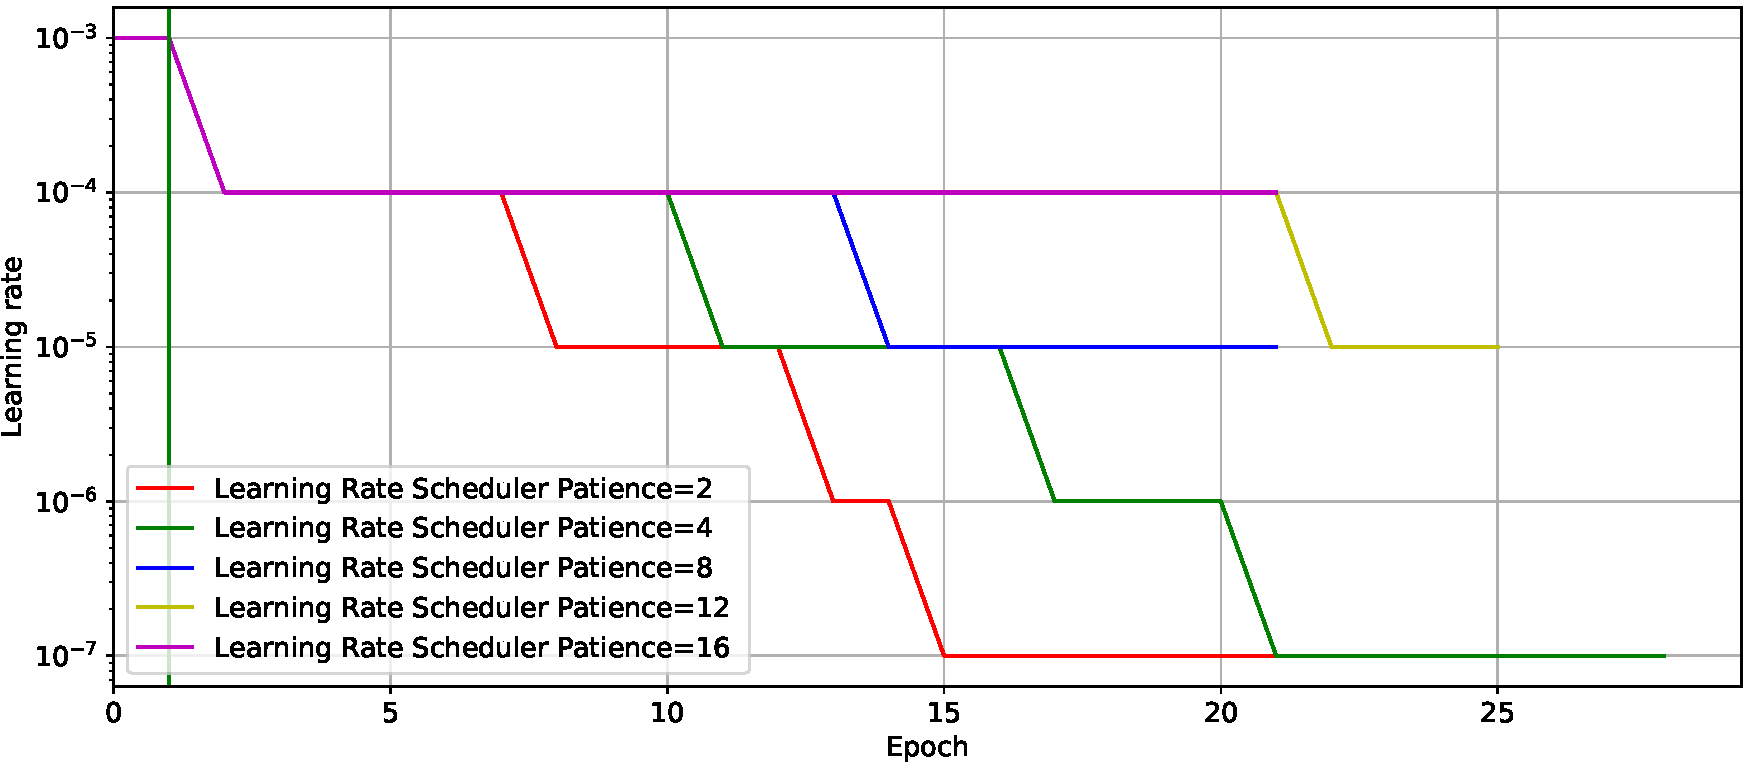
\includegraphics[width=\textwidth]{figs/densenet201_patience_lr_over_epochs.pdf}
        \caption{Influence of the learning rate scheduler's patience on the learning rate over epochs for the DenseNet201 trained with 5000 samples.}
        \label{fig:patience_lr_over_epochs}
    \end{figure}
    
    \subsection{Applying Regularization Techniques}
    From the results in \autoref{fig:patience_bma_over_epochs}, one can see that even for the chosen hyperparameters the model still suffers from overfitting, as seen by the huge discrepancy between training and validation \ac{BMA}. In light of the problem, L2 regularization can help reduce this issue by adding a cost to the loss function of the network for large weights values \cite{Ng}. Presumably, L2 regularization will create an overall simpler model that will be forced to learn only the relevant patterns in the training data.\par
    
    However, results in \autoref{fig:densenet201_lambda_comp} show that the L2 regularization method has a negative impact on the train and validation \ac{BMA} scores. Even though high L2 values reduce overfitting, they also significantly cut the performance values both on train and validation sets. Moreover, small L2 values do not significantly reduce overfitting, while still having a big impact on the generalization performance. Therefore, this method does not seem to be appropriate to reduce overfitting. \par
    \begin{figure}[ht]
        \centering
        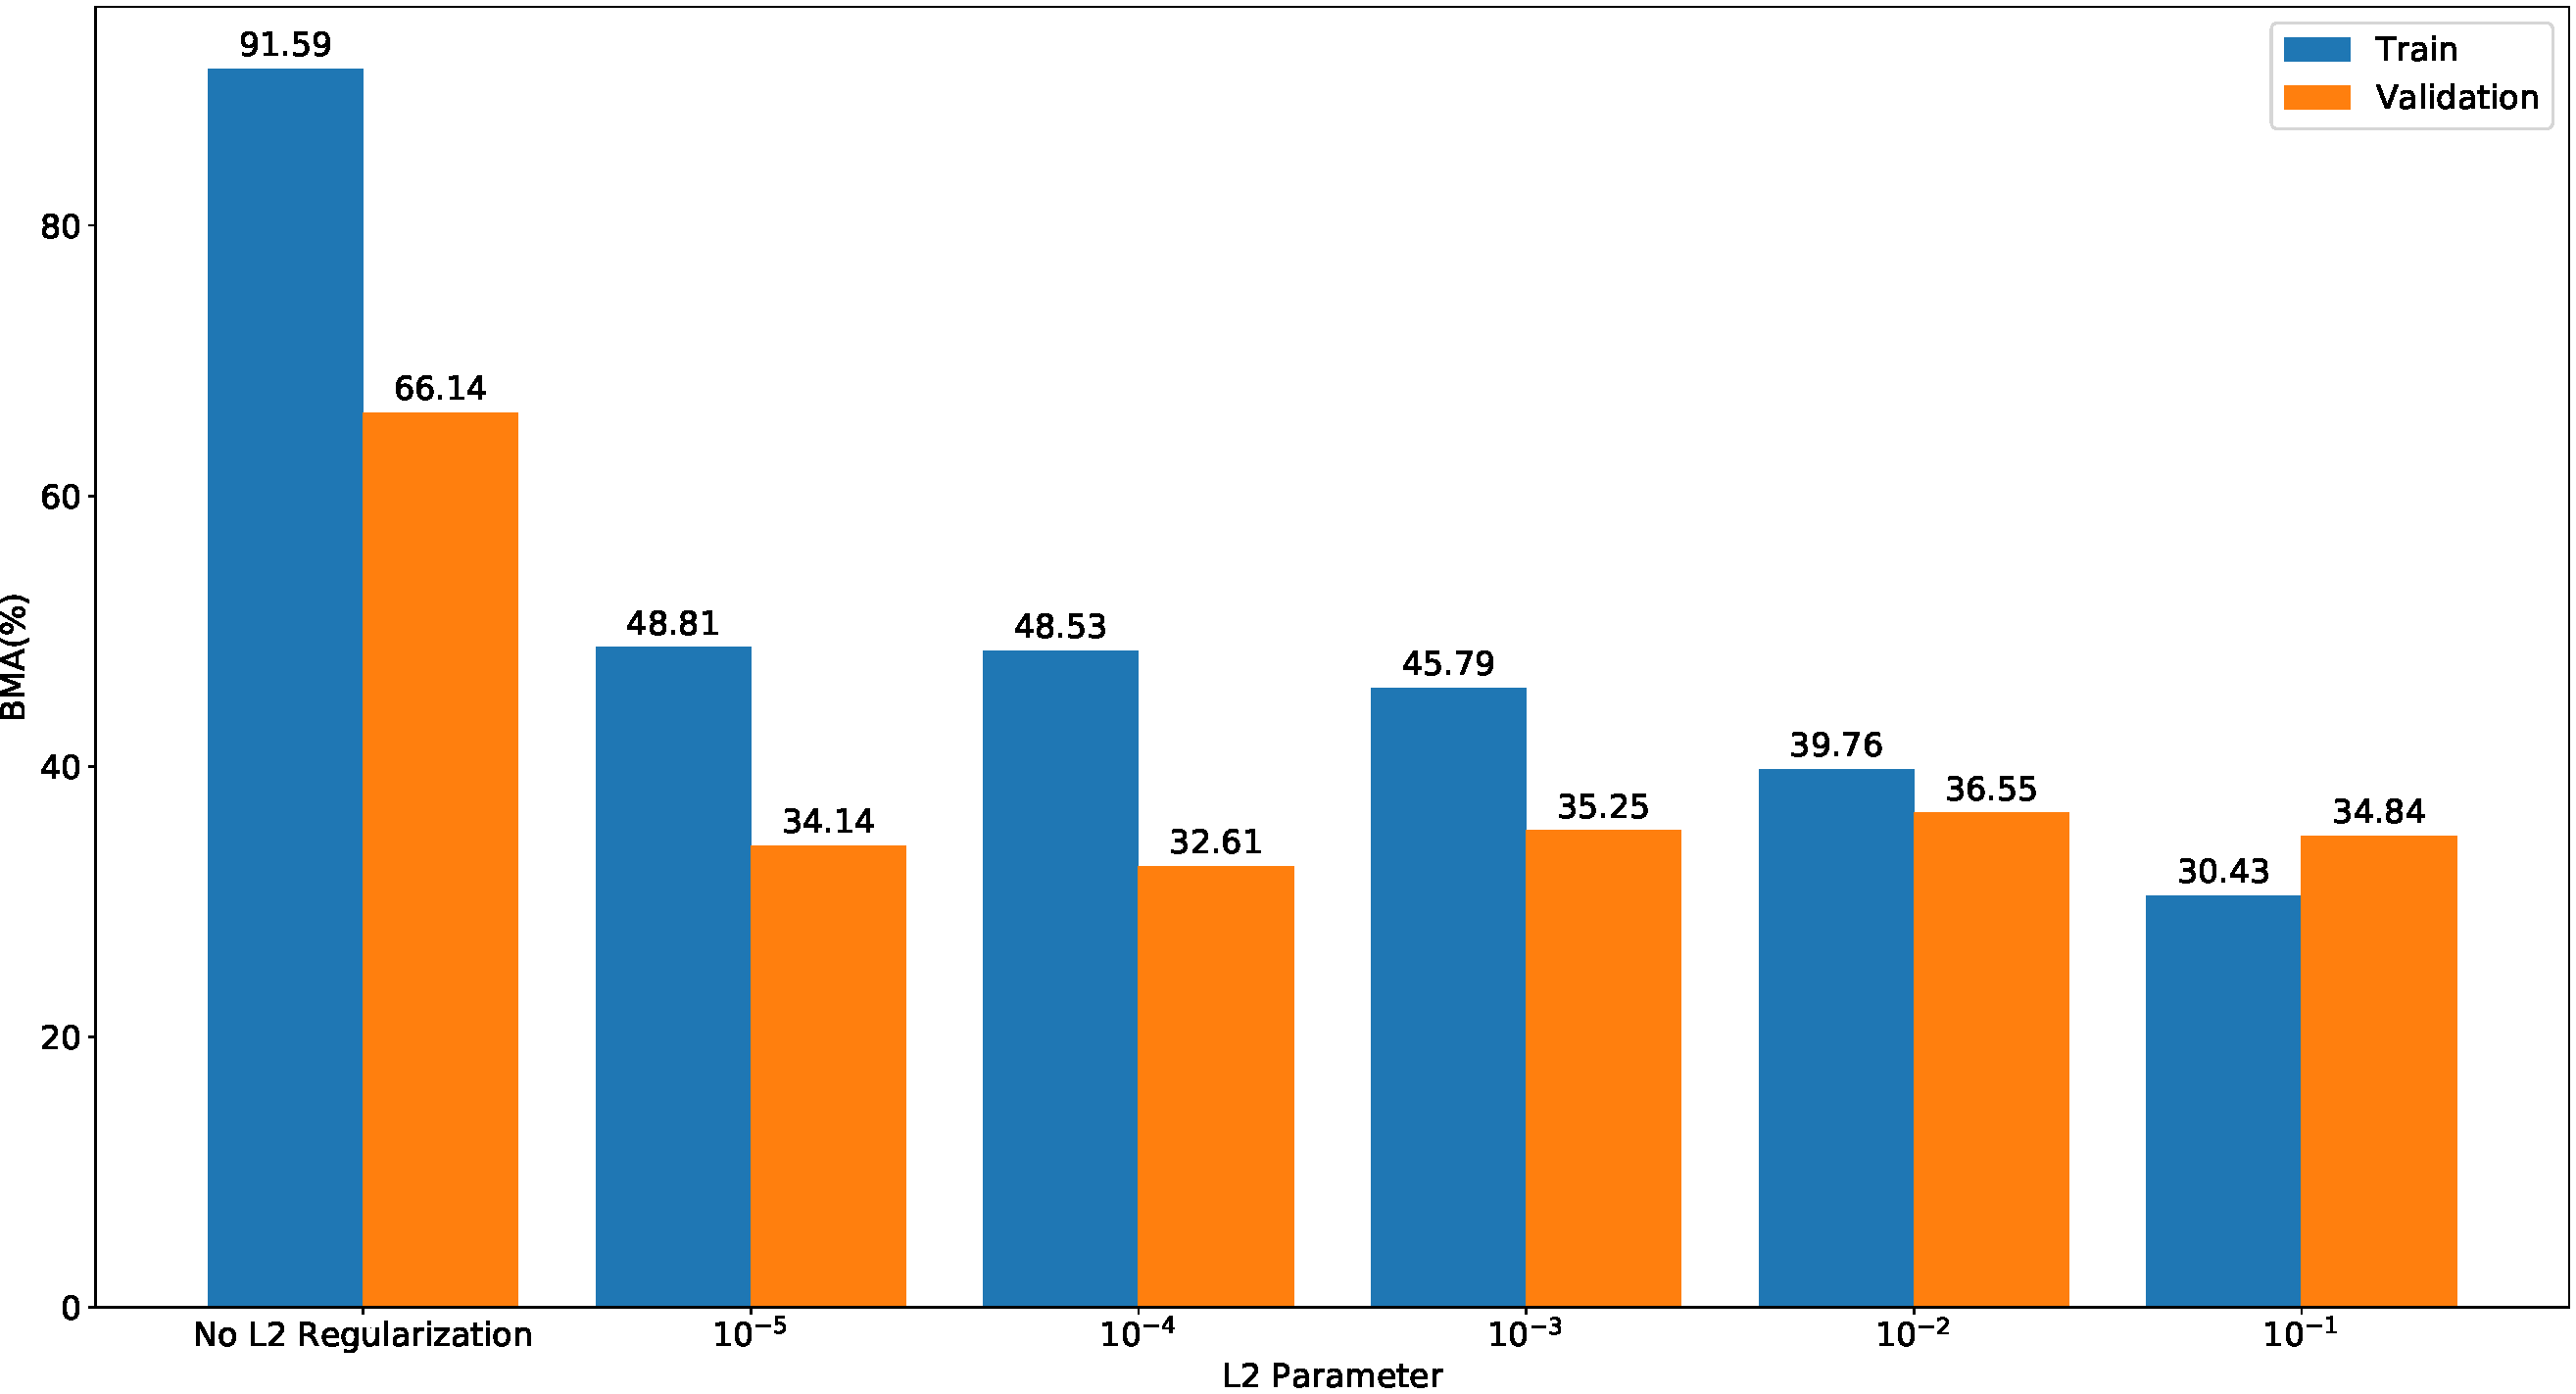
\includegraphics[width=\textwidth]{figs/densenet201_lambda_comp.pdf}
        \caption{L2 regularization parameter vs train and validation \ac{BMA} for the fine-tuned DenseNet201 trained with 5000 samples.}
        \label{fig:densenet201_lambda_comp}
    \end{figure}
    
    Another regularization technique called dropout \cite{Hinton2012} was also experimented with. For this approach, the classifier uses a dropout layer within the classifier, in which the dropout rate is varied. However, results in \autoref{fig:densenet201_dropout_comp} show that adding this method will significantly decrease the train and validation \ac{BMA}. Furthermore, results show that no less overfitting is presented when applying such a technique. Therefore, similarly to the L2 regularization, this method does not seem appropriate to solve this overfitting problem. \par 
    \begin{figure}[ht]
        \centering
        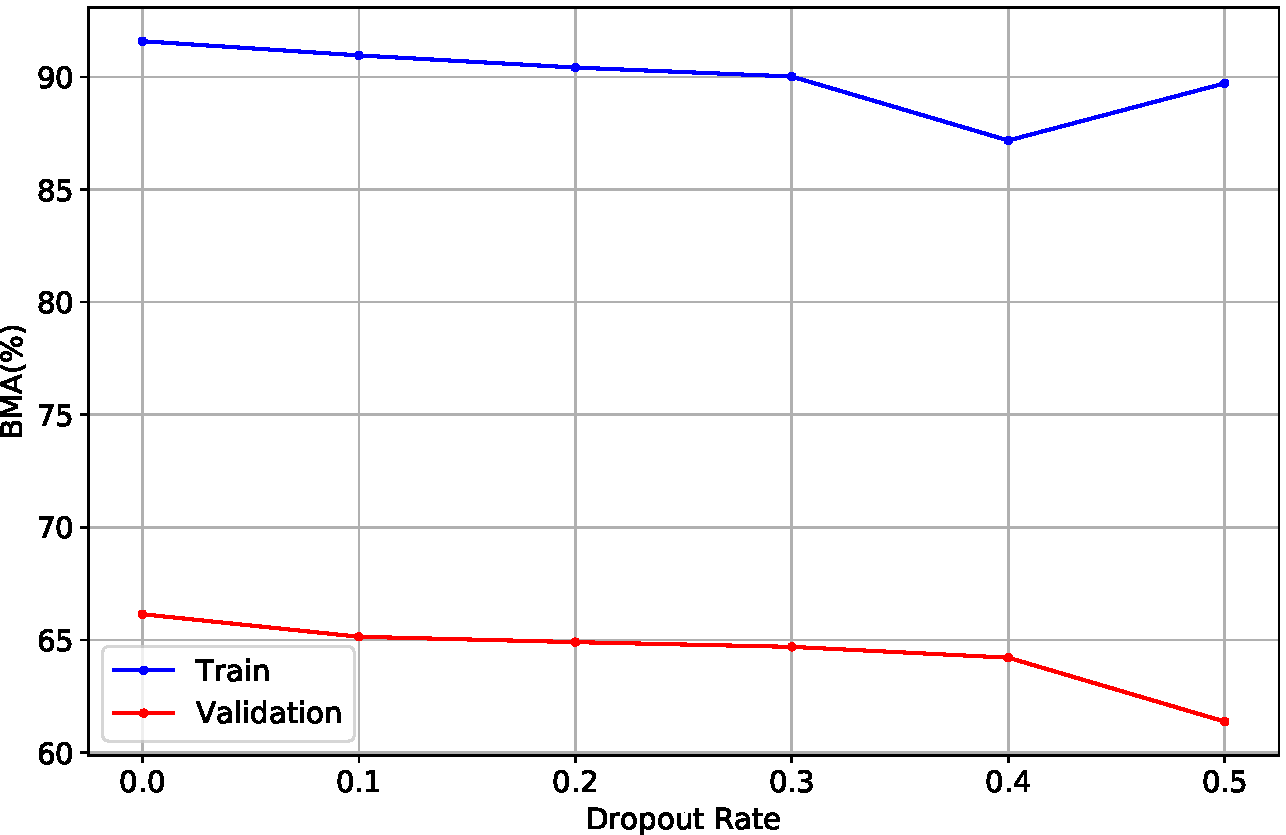
\includegraphics[width=0.7\textwidth]{figs/densenet201_dropout_comp.pdf}
        \caption{Dropout rate vs train and validation \ac{BMA} for the fine-tuned DenseNet201 trained with 5000 samples.}
        \label{fig:densenet201_dropout_comp}
    \end{figure}
    
\section{Results Discussion}
\label{section:optimization_discussion}
    The results of the experimentation of different pre-trained models in \Cref{section:models} found clear support for the presented hypothesis. More specifically, applying transfer learning through fine-tuning the whole set of weights from both the convolutional base and the classifier is a better approach than total parameter extraction without fine-tuning in the context of skin lesion diagnosis. The argument behind these findings is that the dataset used to train those pre-trained models is largely different from the \ac{ISIC} 2019 dataset, which means that those weights need to be adapted for the new dataset. Therefore, these results can be taken as a heuristic for future adaptations of pre-trained models for skin lesion diagnosis. \par
    
    Furthermore, results show that more recent \ac{CNN} architectures such as DenseNet or EfficientNet (see \autoref{tables:pretrainedmodels}) outperform older architectures like VGG or ResNet. Even within the same architecture, variants benefit from the extra number of layers and the extra number of trainable parameters for train and generalization performance. In comparison, pre-trained models like the VGG16 fall behind, presumably because these models lack the ability to create as many levels of abstraction as other networks with more layers. \par 
    
    Moreover, by extracting and fine-tuning the parameters of the convolutional base of the DenseNet201 model trained with a new classifier on top, the model attains a \ac{BMA} score of 0.579 and a accuracy score of 0.746 (see \autoref{fig:pre_trained_model_val_comp}). However, as shown in the confusion matrix of \autoref{fig:densenet201_untuned_conf_matrix}, even this model, which is the best performing pre-trained model, struggles on classification of underrepresented classes such as dermatofibroma (DF), while performing well with overepresented classes such as the melanocytic nevus (NV). \par
    \begin{figure}[ht]
        \centering
        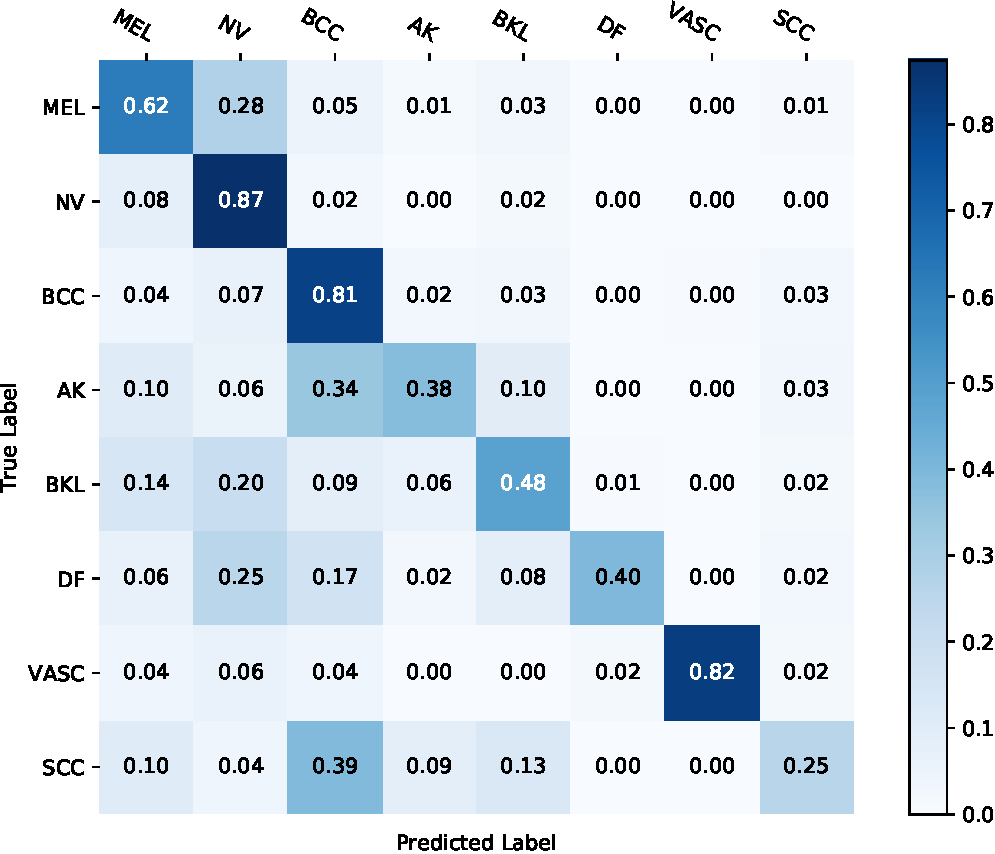
\includegraphics[width=0.7\textwidth]{figs/densenet201_untuned_conf_matrix.pdf}
        \caption{Confusion matrix of the fine-tuned DenseNet201 pre-trained model, trained on 5000 \ac{ISIC} 2019 samples.}
        \label{fig:densenet201_untuned_conf_matrix}
    \end{figure}
    
    While hyperparameter tuning in \Cref{section:hyperparameters} had a small impact on generalization performance, it allowed us to identify key insights about the influence of some of the network's hyperparameters. More specifically, results show that low batch sizes have a regularization effect on the training process, but in turn, extend the training times further. The presented results on the classifier weight updates show very little substantial impact when no updates are applied before the fine-tuning process, which hints that the pre-trained model's classifiers are well adapted to be initialized with conventional methods like Xavier's initialization. \par
    
    Additionally, the importance of the start fine-tuning learning rate was clearly shown in \Cref{section:lr_tune}. Too high fine-tuning learning rates overshoot convergence points and too low learning rates make the weight updates too small which ultimately leads to slow improvements in the training process. However, the learning rate of $10^{-4}$, makes the models converge fast concerning the loss function, which ultimately leads to better \ac{BMA} scores on the validation set. Moreover, one should take into consideration the use of the learning rate scheduler as a method to adapt the learning rate along the training process. In this context, low patiences lead to premature early stopping, high patiences never find good convergence points along with the loss function, but a middle point (\textit{e.g.}, 8) helps the model in the process of finding good convergence spot.
    
    Finally, from the presented results, it is very apparent that there is a high amount of overfitting. Unfortunately this analysis found evidence that regularization methods such as the L2 regularization or dropout are quite ineffective for the undersampled dataset. Even with the hyperparameter tuning, the DenseNet201 model is only able to attain an accuracy of $75.4\%$ and a \ac{BMA} of $59.1\%$ on the test set. The values of the \ac{BMA} are low relative to the accuracy because underrepresented classes have poor performance in comparison with overrepresented classes (this effect is shown in the confusion matrix of \autoref{fig:hyperparameter_tuned_conf_matrix}), which the accuracy metric does not take into account. Therefore, there is a clear need to improve the model's generalization performance, which is the issue that is going to be addressed in \Cref{chapter:experiments2}.\par
    
    \begin{figure}[ht]
        \centering
        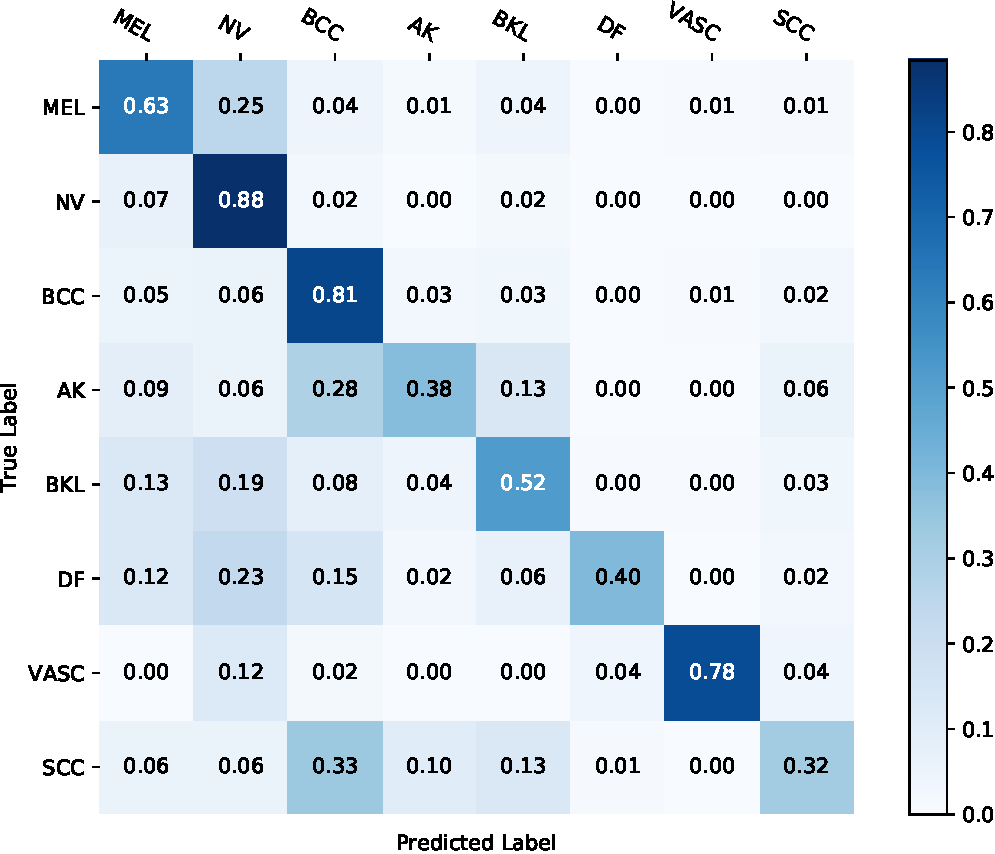
\includegraphics[width=0.7\textwidth]{figs/densenet201_5000_tuned_conf_matrix.pdf}
        \caption{Confusion matrix of the hyperparameter optimized and fine-tuned DenseNet201 pre-trained model, trained on 5000 \ac{ISIC} 2019 samples.}
        \label{fig:hyperparameter_tuned_conf_matrix}
    \end{figure}
